\documentclass[12pt]{scrartcl} %for better layouts
\usepackage{setspace}

\usepackage{graphicx}
\usepackage{amsmath}
\usepackage{natbib} %for citet and citep
\usepackage{syntonly}
%\syntaxonly for quickly checking document

%set document settings
\onehalfspacing % from package setspace

\title{The Effect of Oil Price on Field Production}
\subtitle{Evidence from the Norwegian Continental Shelf}
\author{
  		Johannes Mauritzen \\
        Department of Business and Management Science\\
        NHH Norwegian School of Economics\\
        Bergen, Norway \\	           
		}
\date{\today}

\begin{document}
\begin{spacing}{1} %sets spacing to single for title page
	\maketitle
\end{spacing}

\begin{abstract}
An increase in oil prices could affect oil production in a particular region in three ways.  Higher oil prices could lead to increased exploration, starting production in known but previously uneconomic fields or to changes in production in existing fields.  While several studies exist on the effect of oil prices on exploration, to my knowledge no studies exist of the effect of oil price on production in existing fields.  I use detailed data on Norwegian oil field production and a semi-parametric additive model to control for the production profile of fields.  I find no significant evidence of a concurrent reaction of field production to oil prices, though a slight lagged effect is found of the magnitude of approximately 2 to 4\% for a 10 dollar per barrel increase in the real price of oil.  These findings are consistent with the idea of producers that do not act strategically to short-term price movements but instead use storage and financial derivatives to hedge oil price changes.  
\end{abstract}





\section{Introduction}

For most of the last century, crude oil has been the single most important and valuable fuel source in the world.  Naturally, questions of how the oil price affects the world economy as well as how oil production reacts to the oil price have been fundamental topics in economics. However a significant gap exists in the literature.  While several studies have taken up the issue of how oil prices affects searching for new fields, to my knowledge no field-level studies exist of the effects of oil prices on oil production at existing fields.  

The effect of oil prices on existing field level production is an important topic, both as an empirical counterpart to the extensive theoretical literature on optimal extraction and more generally in understanding the mechanisms of how total oil supply reacts in response to price.  

The lack of research on the role of price in oil field production is likely due to two main factors - the availability of data and the non-linear time profile of field production.  Most oil production has historically either been done by large private oil companies, notably “super majors” and, over the last several decades, by state-owned oil companies and national monopolies.  Both of these types of entities tend to consider field-level data as either company or state secrets.   

Luckily a notable exception to the general rule of inaccessible data exists.  The Norwegian government has committed itself to transparency in the petroleum sector and detailed data sets on most aspects of the country’s oil industry is openly available.  I use historical production data from all 77 currently or formerly oil-producing fields on the Norwegian continental shelf in order to estimate the effect that prices have on oil production.  

By looking only at the effect of price on fields that currently or previously have produced oil I am limiting the scope of this article.  The effect of oil prices on total production over an extended period of time is likely due not just to reactions in production in existing fields but also increased searching for new fields.  In fact, an implication of this work is that much of the total production response from higher oil prices is from increased searching as well as production from previously un-economic fields.

The main finding in this article is that oil production at the field level has no significant reaction to concurrent changes in the oil price, where concurrent is broadly defined as within the first three years.  A slight effect can be detected at a lag of between 4 and 6 years, with a magnitude of about a 2 to 4\% increase in yearly production for a 10 dollar increase in the price of oil.  This effect is somewhat greater and with less of a lag in large fields compared to small fields.

The main methodological problem, as mentioned, is the non-linear production profile of oil fields.  Once full scale extraction is started in an oil field, pressure in wells will quickly drop.  Technological solutions such as gas and water injection also have quickly declining effectiveness.  In turn production will drop quickly. 

Oil field production is correlated across fields - that is, increases and decreases in production in fields are not randomly distributed across time.  Instead, as figure \ref{top10_production} shows with the production profile of the 10 largest Norwegian oil fields, production tends to be correlated across fields.  The result is a total production curve that is bell shaped over time as figure \ref{oil_decline}  shows.  Since oil prices are autocorrelated, a failure to properly account for the production profile will lead to spurious estimation of the price terms in a regression.  

The direction of this bias can be gleaned in figure \ref{oil_decline}.  High oil prices were present at periods of relatively low production in the late 1970s and early 1980´s as well as the last 10 years, however real prices reached some of their lowest levels at the same time as the top of production around the year 2000.  This inverse relationship is of course entirely accidental, but will heavily bias the estimation of the effect of price on production if the production profile at the level of the oil field is not properly accounted for.  

\begin{figure}
	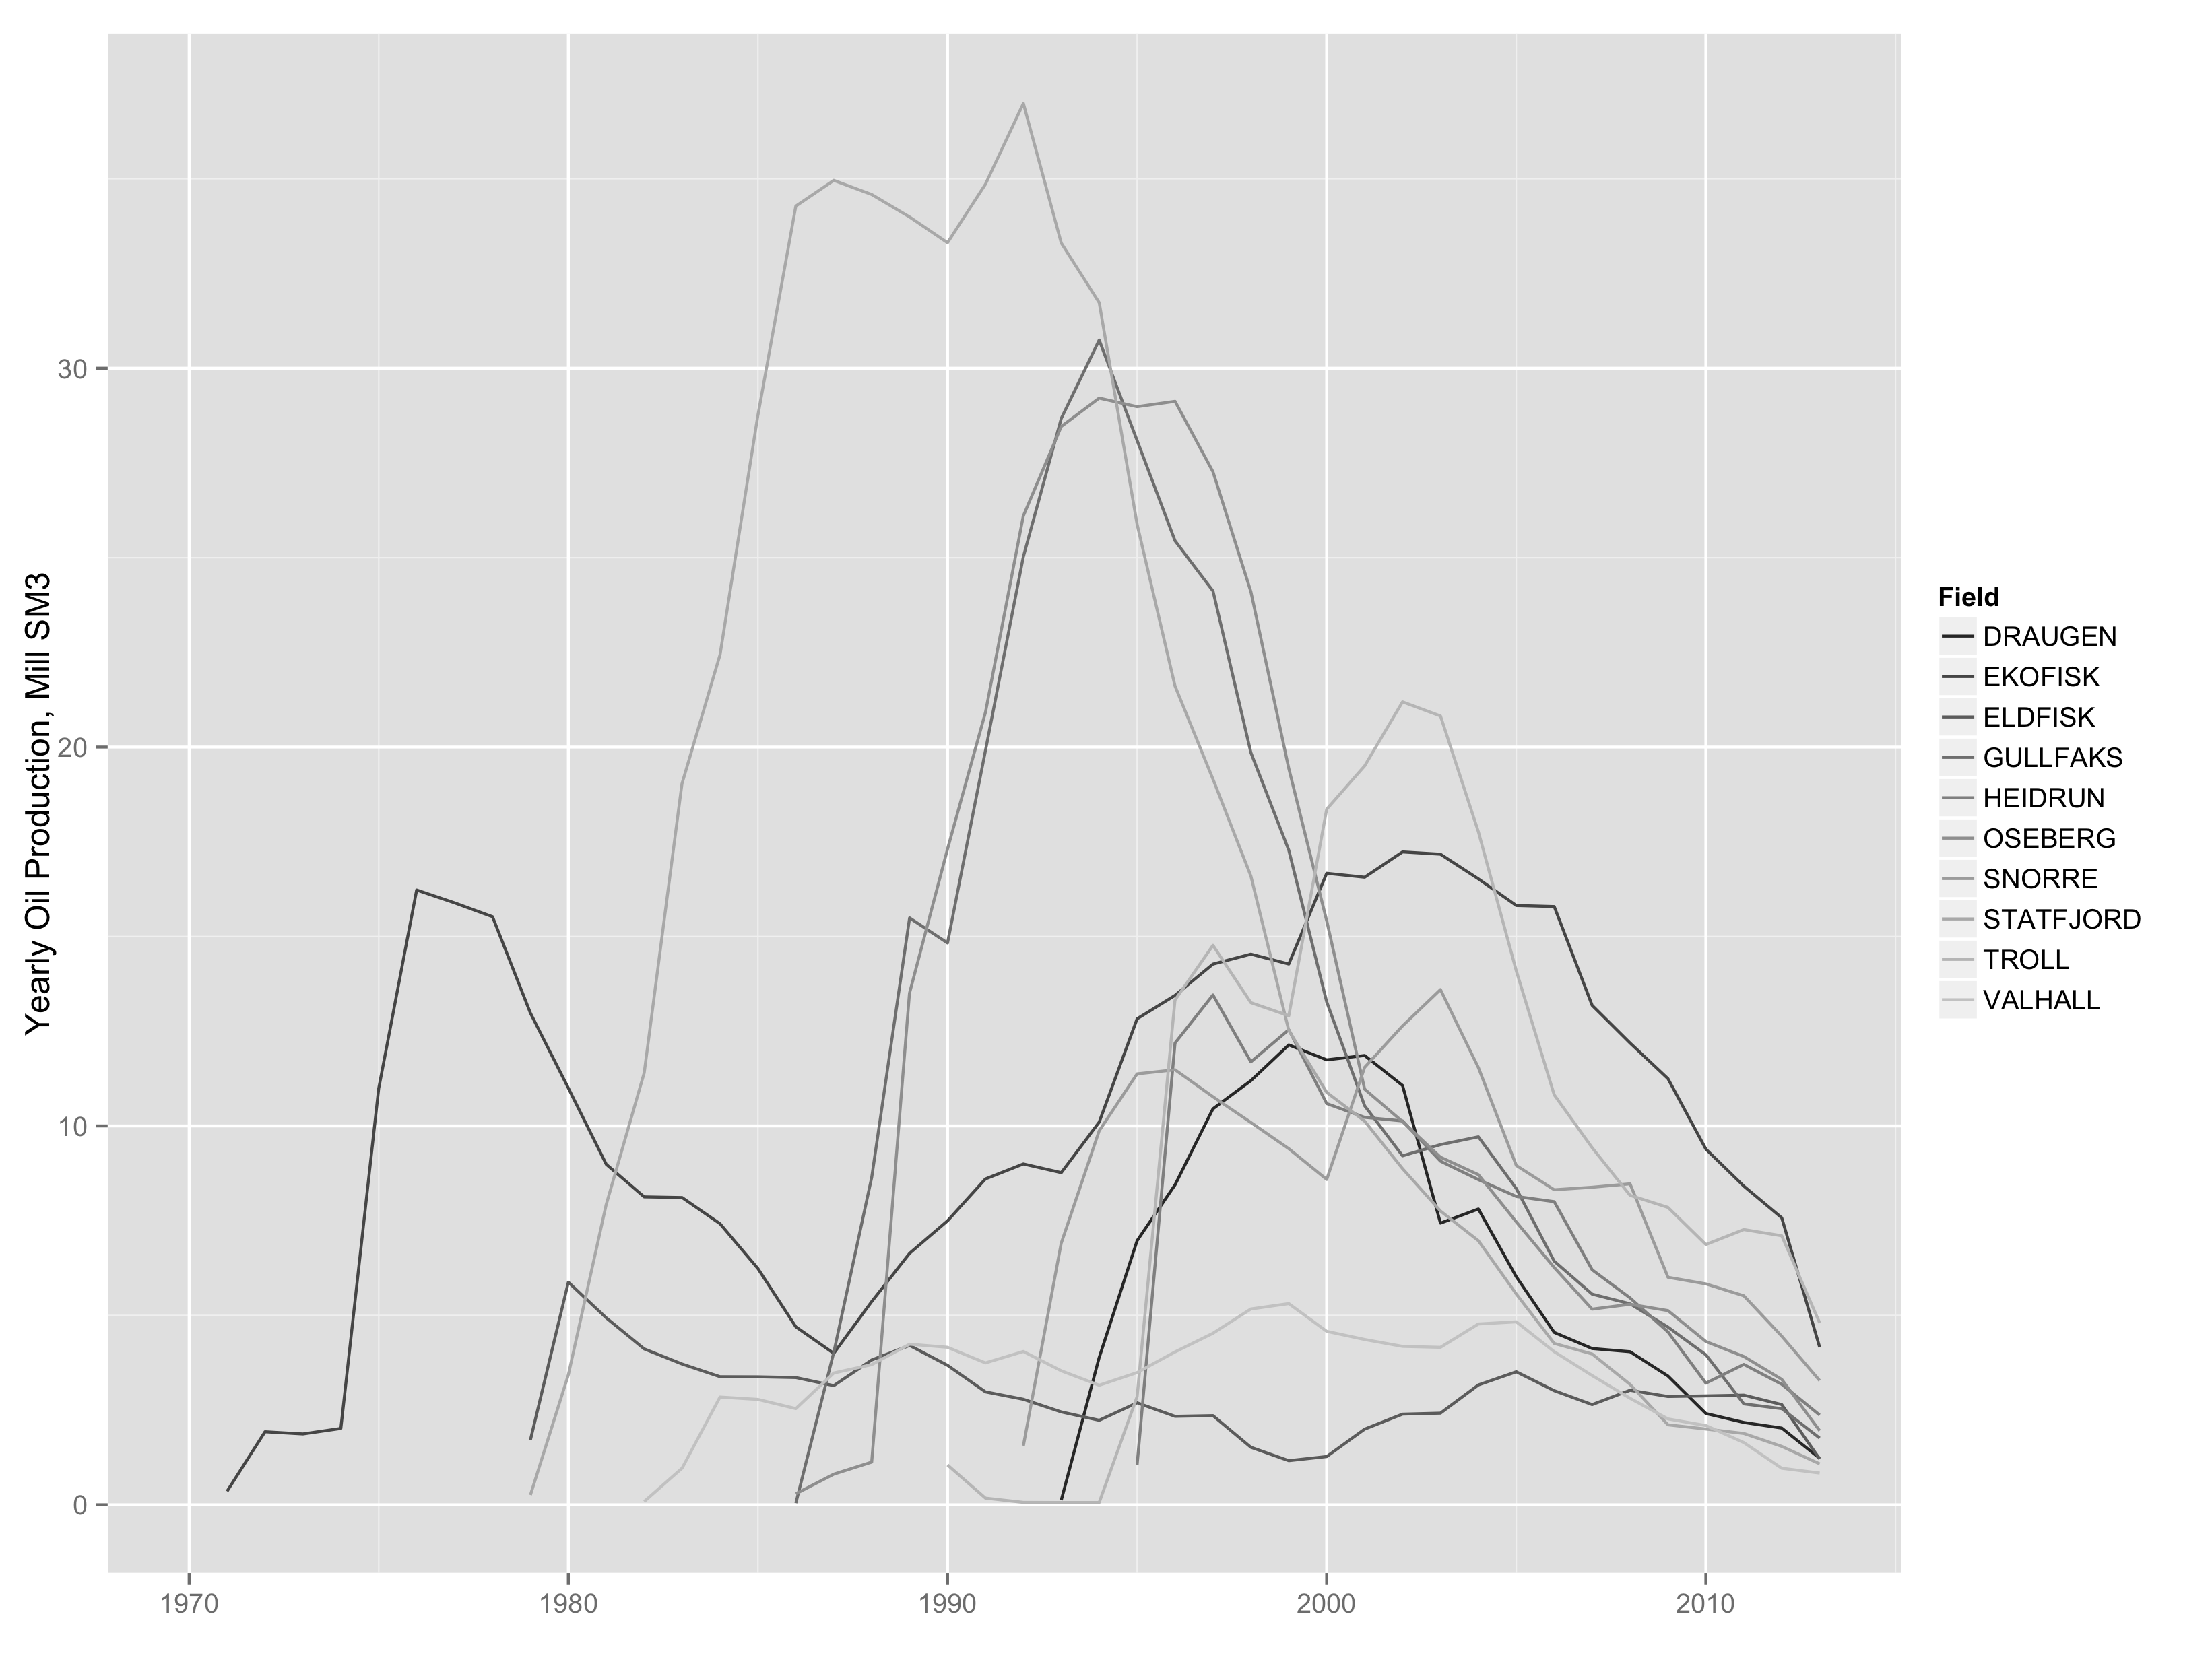
\includegraphics[width=.8\textwidth]{top10_production.png}
	\caption{}
	\label{top10_production}	
	\end{figure}

\begin{figure}
	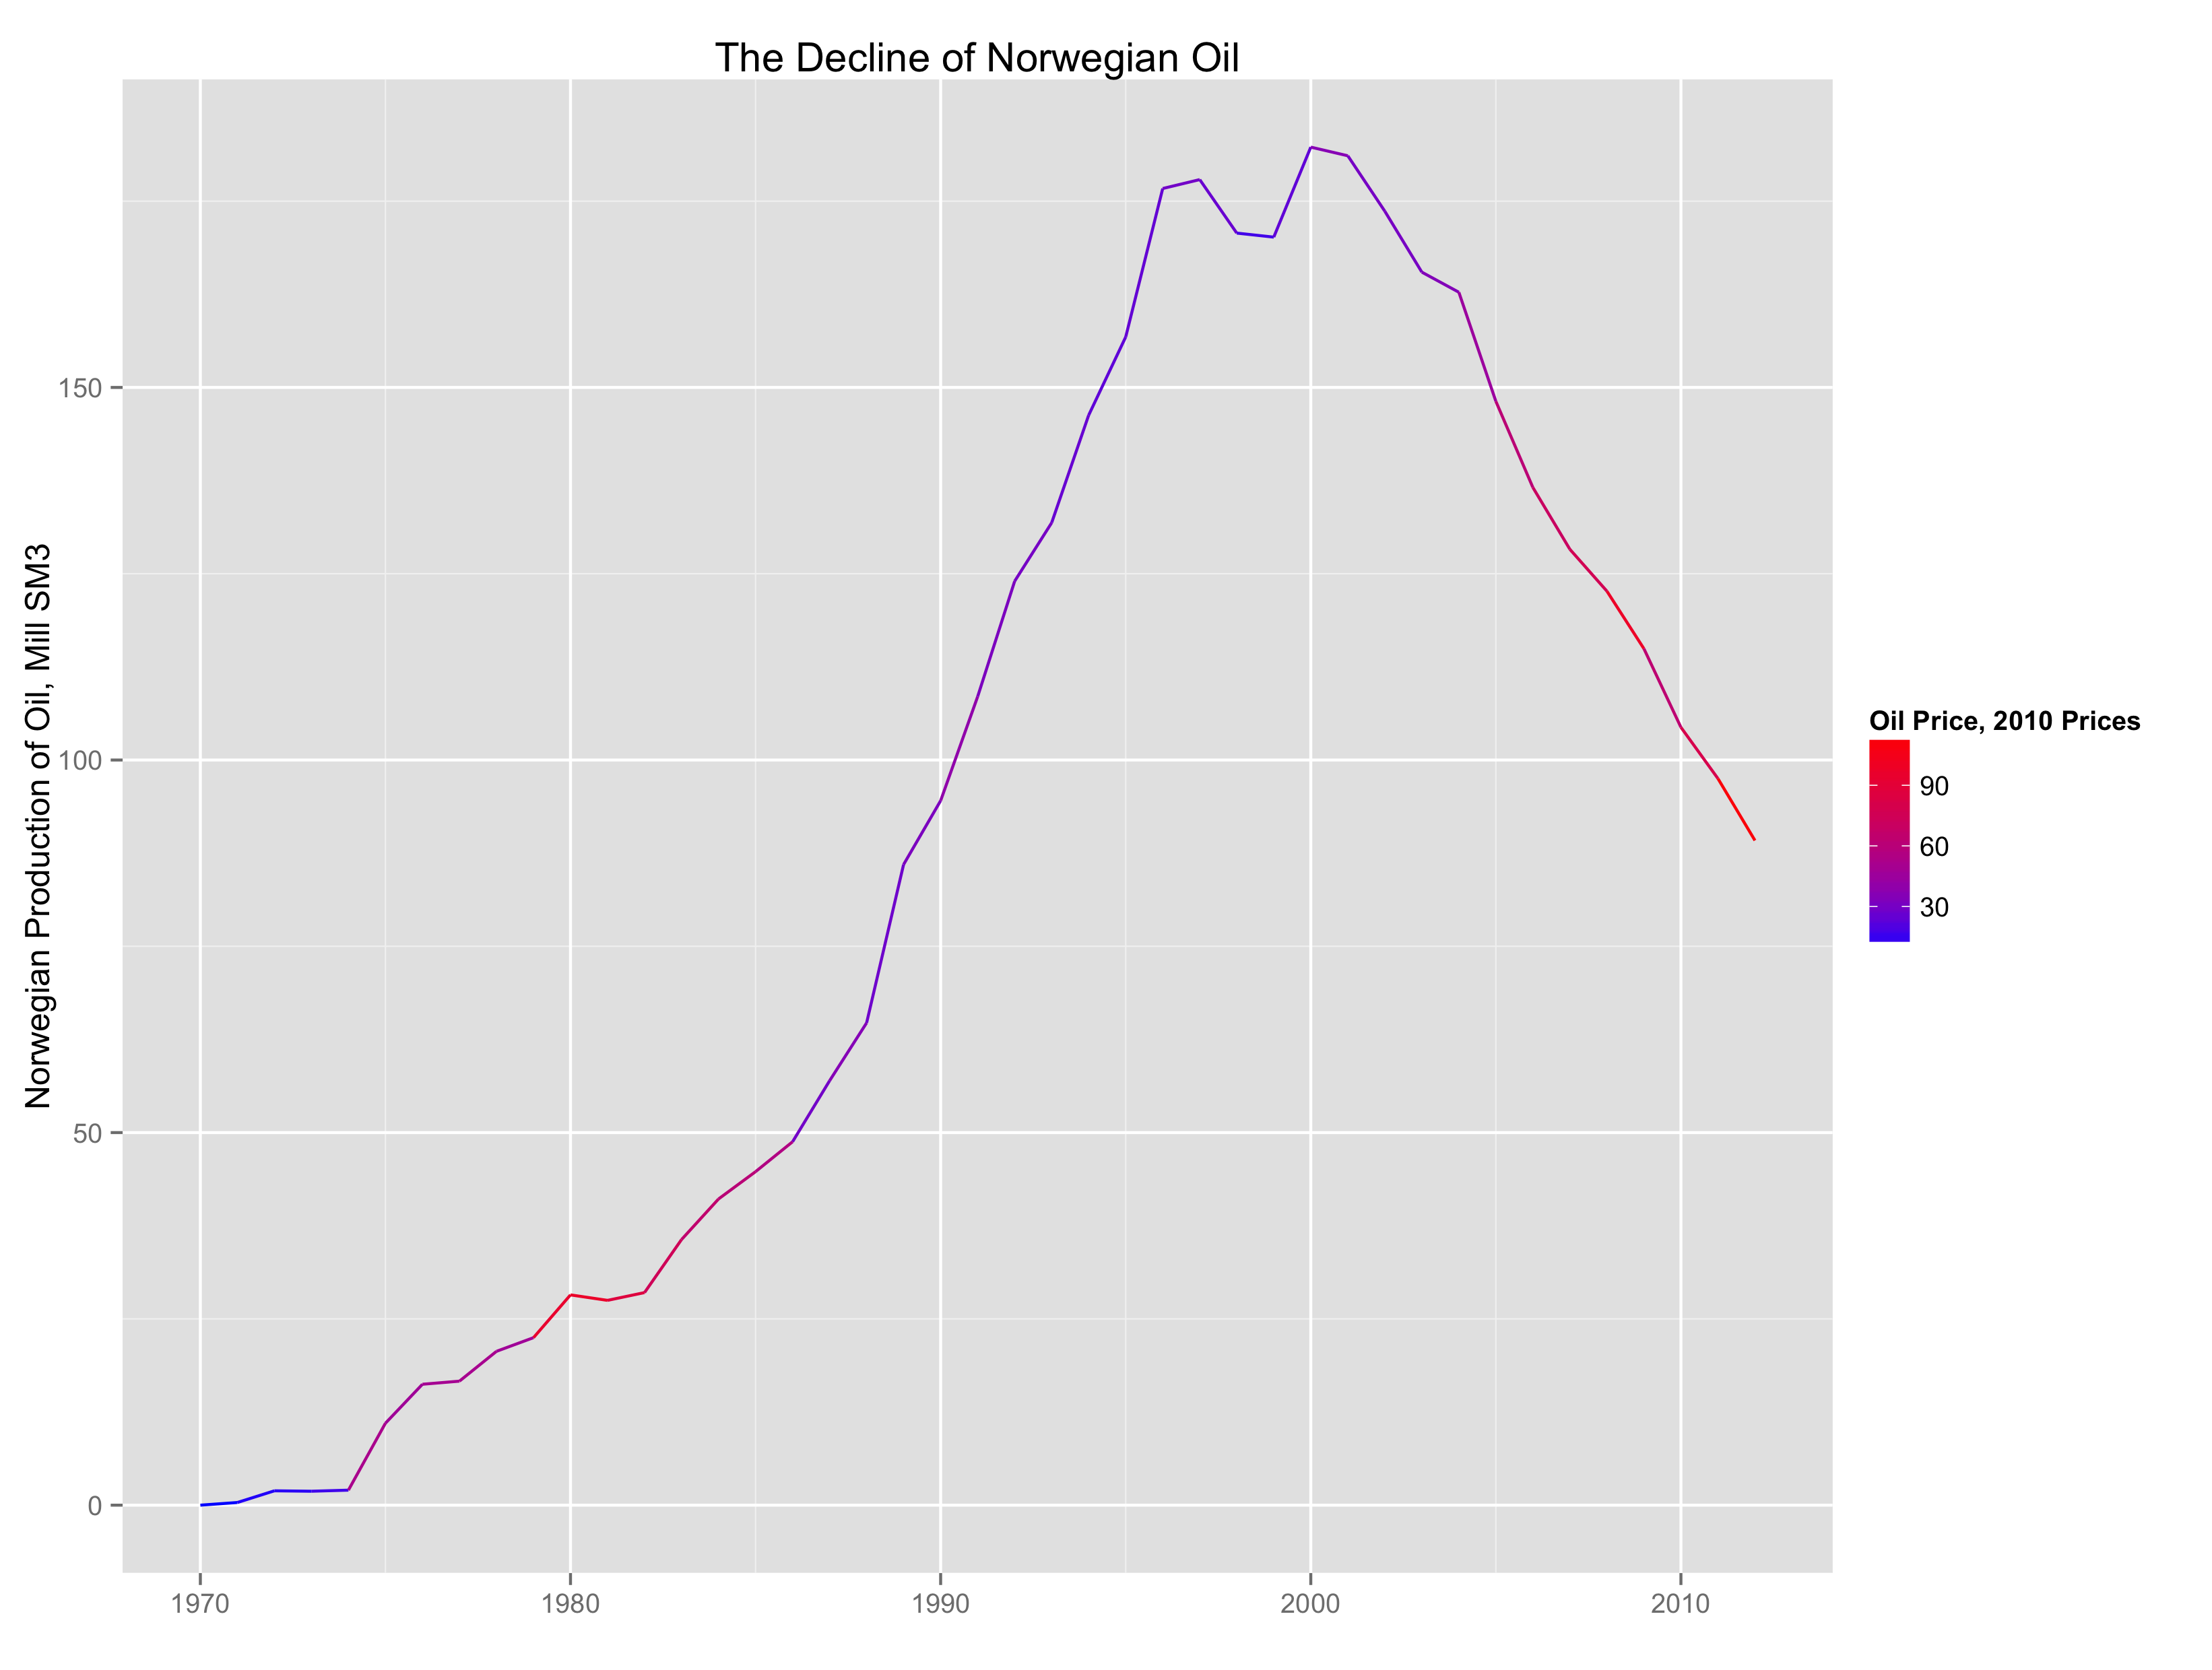
\includegraphics[width=.8\textwidth]{oil_decline.png}
	\caption{}
	\label{oil_decline}
\end{figure}

As a solution I use a semi-parametric model within the Generalized Additive Model frameworks of \cite{hastie_generalized_1990}.  Here I use a two-dimensional smoothed spline function to account for the general non-parametric shape of the production profile.  The coefficient on the price variable can then be seen as the average price effect.  

\section{The effect of oil price on production: theory and empirics}
The question of the effect of oil prices on production and the more general question of optimal oil extraction has a long history and goes back to the seminal work of \citet{hotelling_economics_1931}.  The theoretical literature on optimal extraction is too vast to cover even at a superficial level, however \citet{krautkraemer_nonrenewable_1998} provides a good overview.  More important to this paper have been empirical estimates of the effect of price on production.  \citet{black_is_1998} Presents a more recent test of whether oil prices have an effect on oil production or whether production is purely determined by geo-engineering factors.  The authors find strong evidence of a role of price using data from seven montana oil fields, but their model does not allow for an estimation of magnitude.  

Several papers seek to answer the question of how aggregated oil supply is affected by oil prices.  \citet{farzin_impact_2001} attempts to estimate an elasticity for the effect on added reserves of increased oil prices and finds a small though statistically significant effect.  \citet{ramcharran_oil_2002} estimates a supply function for the total supply of oil from OPEC countries based on data from 1973 to 1997.  The author finds a negative price elasticity, and interprets this as evidence of producers targeting revenue.  However since the author does not take into account geo-engineering factors that will likely affect oil prices, this conclusion comes under considerable doubt.  \citet{boyce_exploration_2011} look at exploration and development of oil fields in the US and using a dynamic model and using state-level data from the US between 1955-2002, conclude that hotelling scarcity effects dominate.  \citet{hamilton_oil_2012} presents a historic description of oil production over time, emphasizing that field-level declines in production are difficult if not often impossible to reverse even given high oil prices.  

the effect of oil-price uncertainty on investments in new and existing production has also been explored.  \citet{kellogg_effect_2010} finds that oil exploration firms in Texas do approximately respond as real-option theory would predict when it comes to the timing of drilling.  A model and test using data from North Sea producers on the UK continental shelf by \citet{hurn_geology_1994}, on the other hand, fails to find evidence that the variance in the oil price affects the timing of oil field development.  

Studies using detailed Norwegian data also exist.  \citet{mohn_exploration_2008} find that long-term changes in the oil-price has a strong effect on exploratory drilling though little effect is measured from short-term changes in the oil price.  \citet{osmundsen_exploration_2010} analyses drilling productivity over time on the Norwegian Continental Shelf while \citet{mohn_efforts_2008} finds that higher oil prices leads to higher reserves by way of both greater efficiency in searching as well as greater effort.  

\section{Oil production on the Norwegian continental shelf}
The first commercial oil well in Norwegian continental waters was discovered in december of 1969 in what became the Ekofisk oil field, the largest Norwegian oil field by estimated recoverable reserves.  As figure \ref{north_sea_reserves} shows, most of the largest fields in the North Sea were found relatively early on while more recent finds have tended to be smaller.  A major exception to this trend was the recent find of the Johan Sverdrup field which is estimated to have approximately 300 million SM3 of recoverable oil. \footnote{The Johan Sverdrup field is estimated to begin producing oil in 2017 and so is not present in data set used for the analysis.}  

\begin{figure}
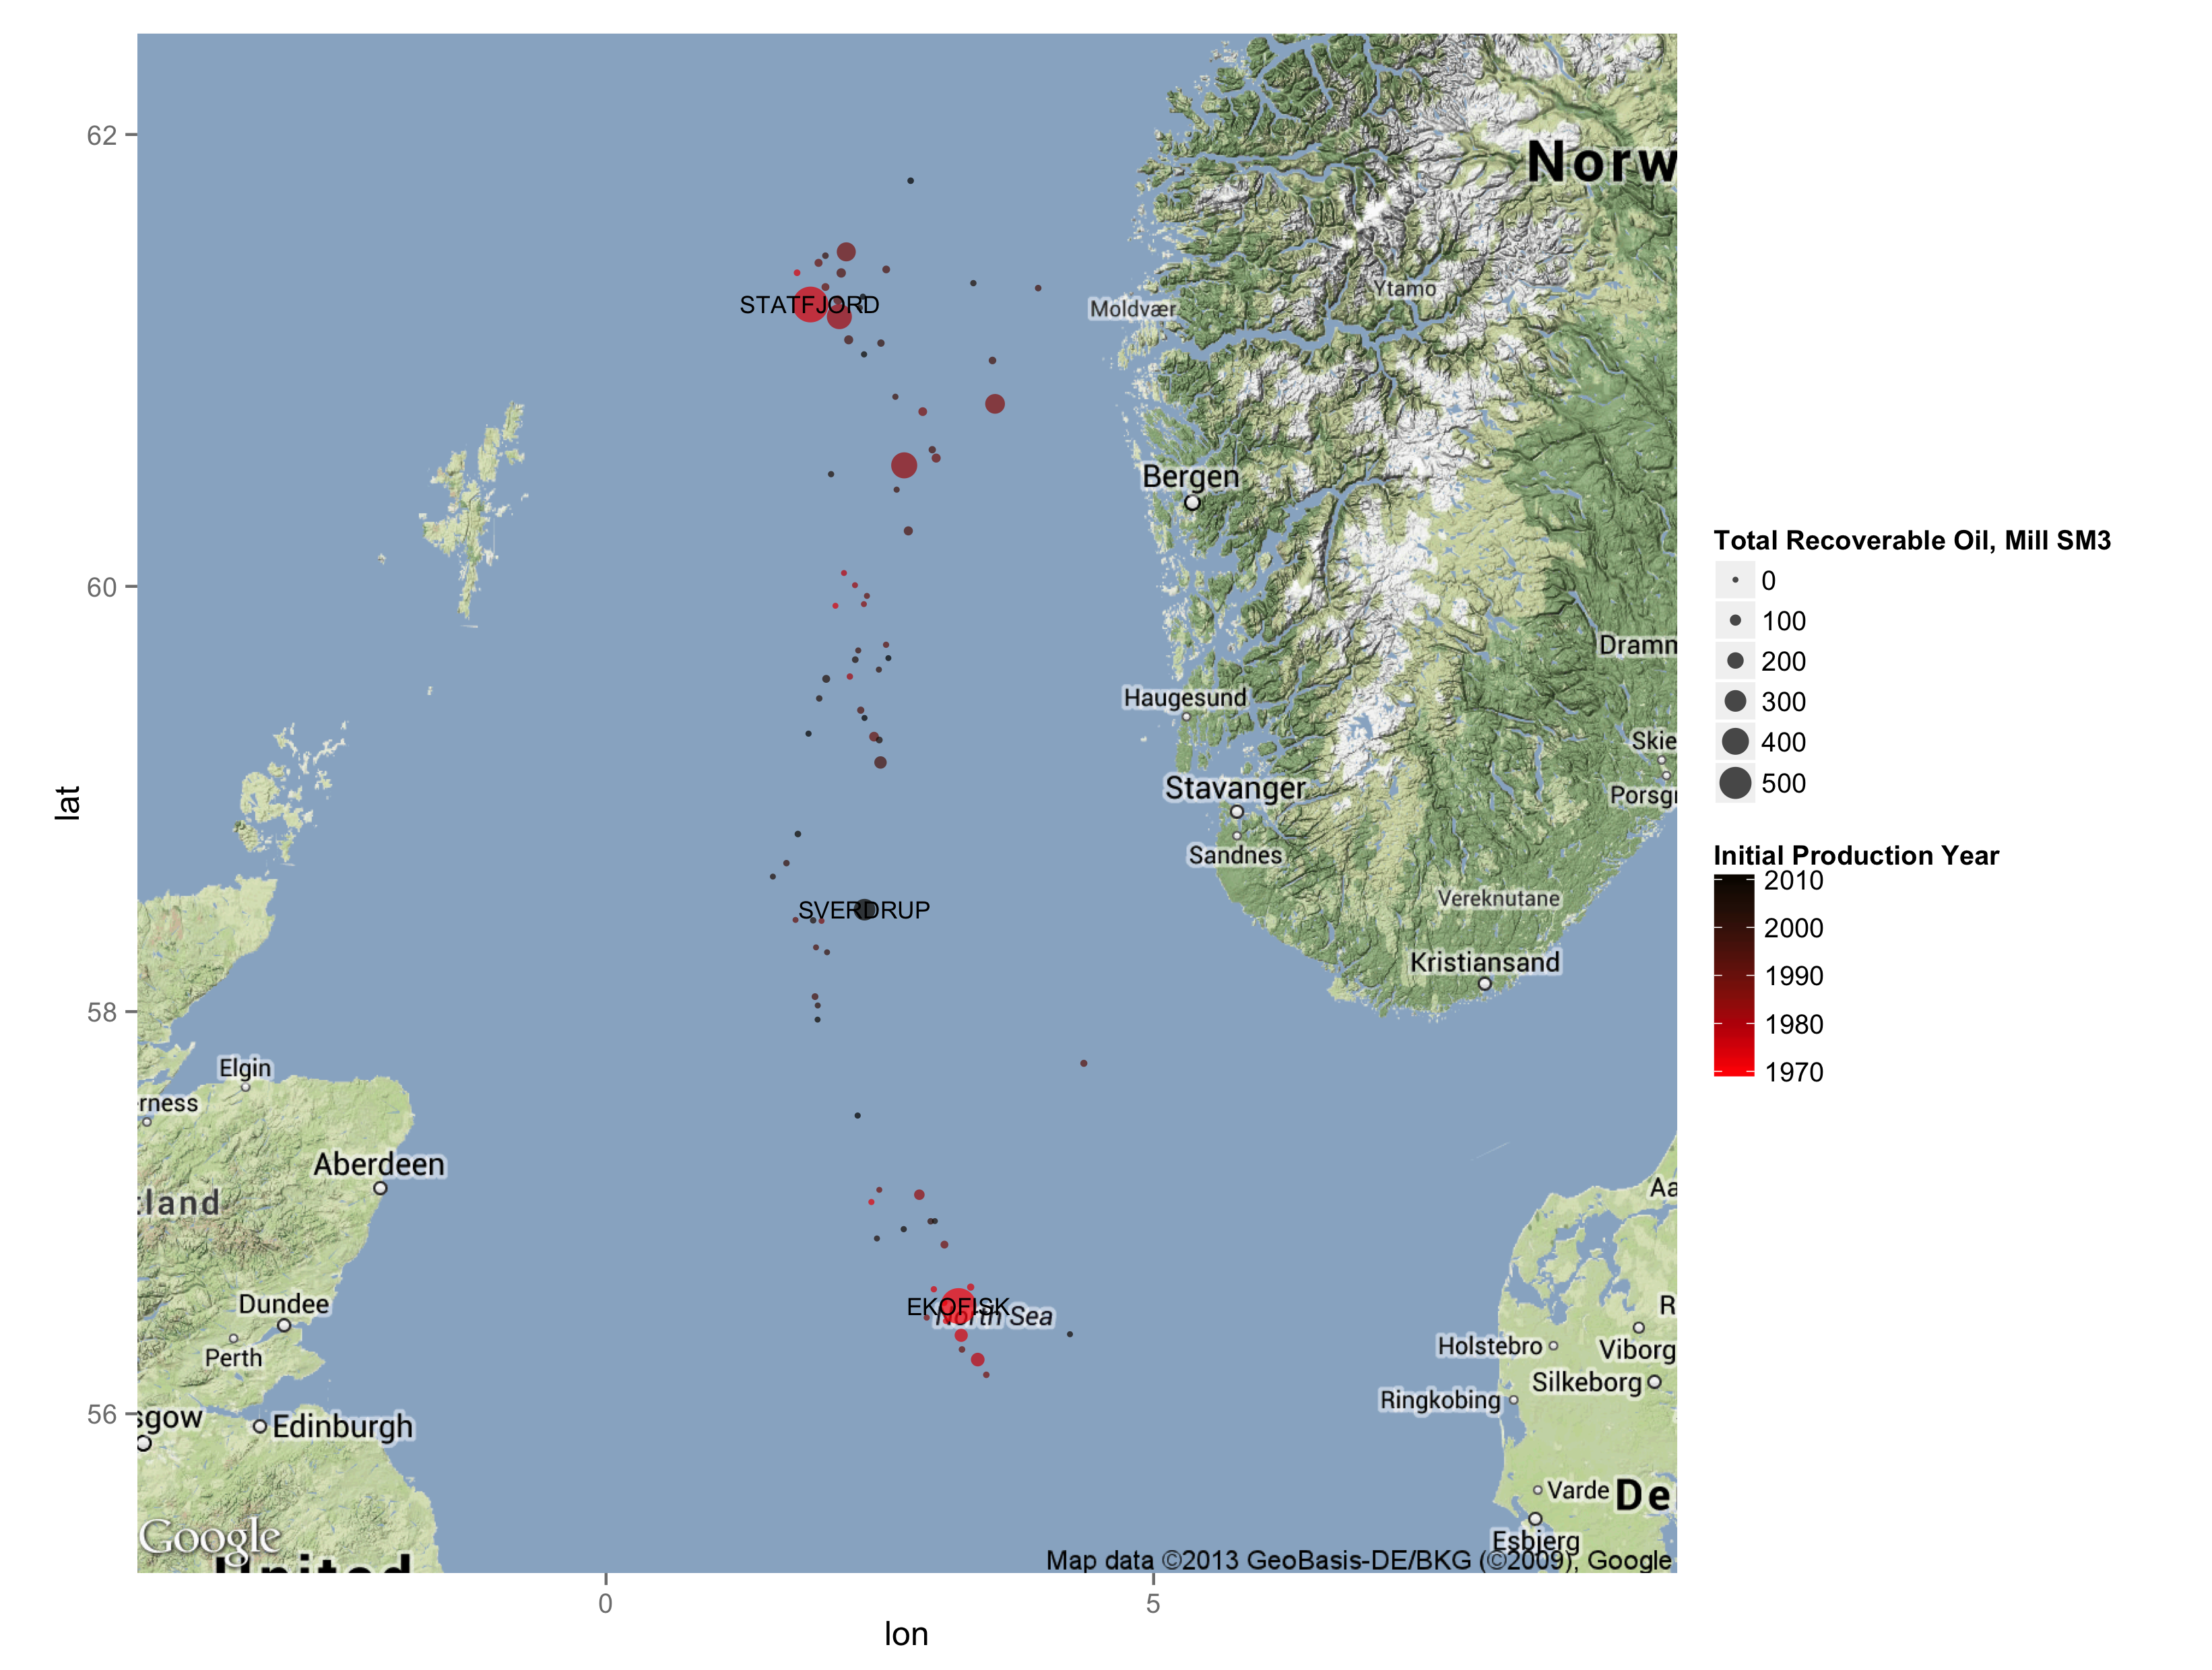
\includegraphics[width=.8\textwidth]{north_sea_reserves.png}
\caption{}
\label{north_sea_reserves}
\end{figure}

Exploration in the Norwegian sea was opened up for exploration in 1980 and the first commercial field started production in 1981.  While several mid-sized fields have been discovered, the Norwegian Sea has generally disapointed in terms of commercial oil finds and most finds have been relatively small (\ref{norwegian_sea_reserves}).  

\begin{figure}
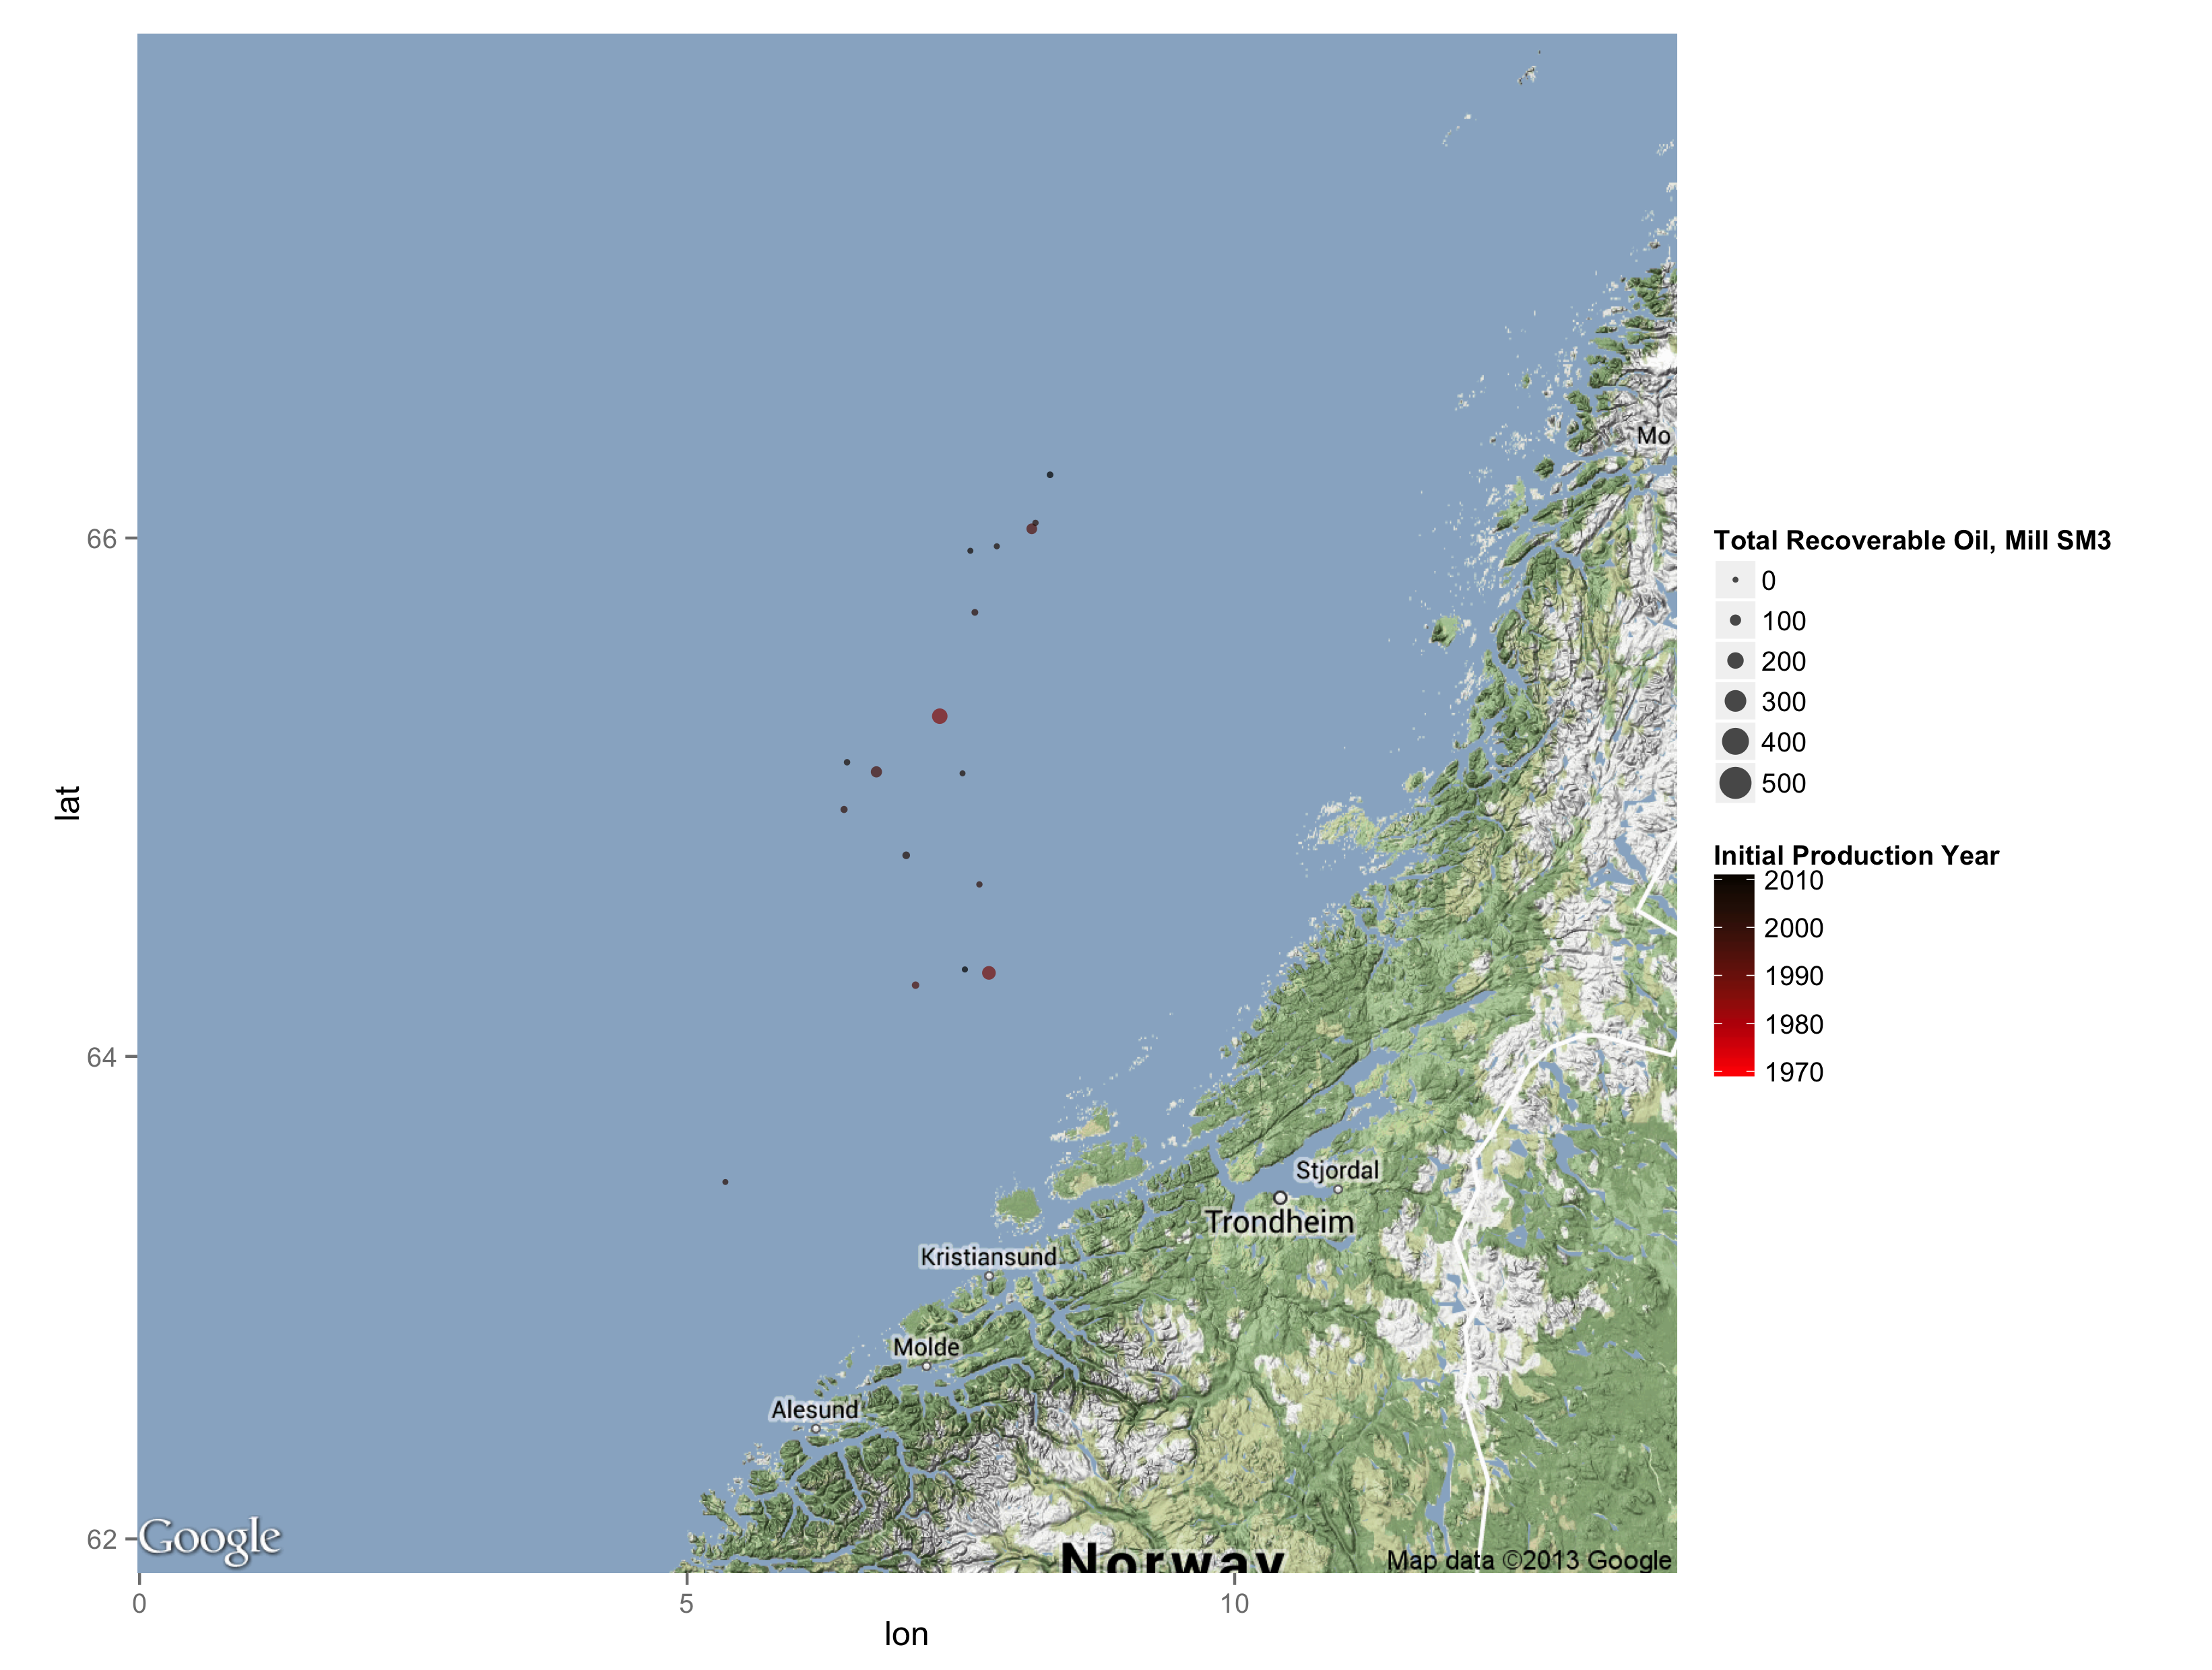
\includegraphics[width=.8\textwidth]{norwegian_sea_reserves.png}
\caption{}
\label{norwegian_sea_reserves}
\end{figure}
Norwegian waters in the Barents sea have also been open to exploration since the 1980s, however up until recently only a few, small finds were made and none came into commercial production.  However more recently several large oil and gas finds have been made in the Barents Sea - notably the oil find Goliat and the large gas find Snøhvit, which are both currently under development but not yet producing.  The agreement between Norway and Russia in June 2011 settling a long-running dispute over the maritime delimitation has also given a boost to new exploration in the region.  

\section{Norwegian oil field production data}
Production data of Norwegian oil fields is obtained from the website of the Norwegian Petroleum Directorate \footnote{http://factpages.npd.no/}  Production data is available at a monthly frequency for all fields, though I choose to aggregate up to yearly values both to smooth over seasonality as well as random changes in output.  

In addition to data on field-level production, I also make use of data on estimated total recoverable reserves.  The use of this variable is complicated as it is an estimate subject to a large amount of uncertainty, especially in relatively young fields.  

I use yearly data from the US Energy Information Agency on the real price of Brent-traded oil in 2010 dollars.  The Brent benchmark oil price is likely the best oil price measure for Norwegian production as it is based on light sweet crude oil sourced from the North Sea.   

\section{A generalized additive model of oil field production}
A parametric linear model has the sizeable advantages of simplicity and interpretability and therefore usually a good starting point for an analysis.  However, when attempting to model the effect of price on oil field production, a standard linear model is unable to sufficiently control for the production profile and therefore biasing the estimate of the effect of price.  As an example, consider a generalized linear model written as in equation \ref{glm_eqn}. 

	\begin{equation}
	\begin{split}
	 Log(Production_{i,t}) & = \alpha_0 + \alpha_1 time\_to\_peak_{i,t} + \alpha_2 time\_to\_peak_{i,t}^2 \\
	& \quad + \alpha_3 time\_to\_peak_{i,t}^3  + \alpha_4 peak\_to\_end_{i,t} + \alpha_5 peak\_to\_end_{i,t}^2 \\
	& \quad + \alpha_6 peak\_to\_end_{i,t}^3 + \gamma total\_recoverable\_oil_i \\
	& \quad + \beta_1 oil\_price + \beta_2 oil\_price\_l1 + ...+ \epsilon
	\end{split}
\label{glm_eqn}
	\end{equation}

Here the left hand side variable is yearly production in year $t$ for field $i$.  To try to account for the time profile of production, I split up model time into a time-to-peak and peak-to-end variable as shown in figure \ref{statfjord_dem} and then represent each as a cubic function.  The total size of the field will of course also play a role in the production and this is added linearly in the model.  Finally, a term for the oil price as well as 5 lagged terms are added in order to capture the effects of price.  

\begin{figure}
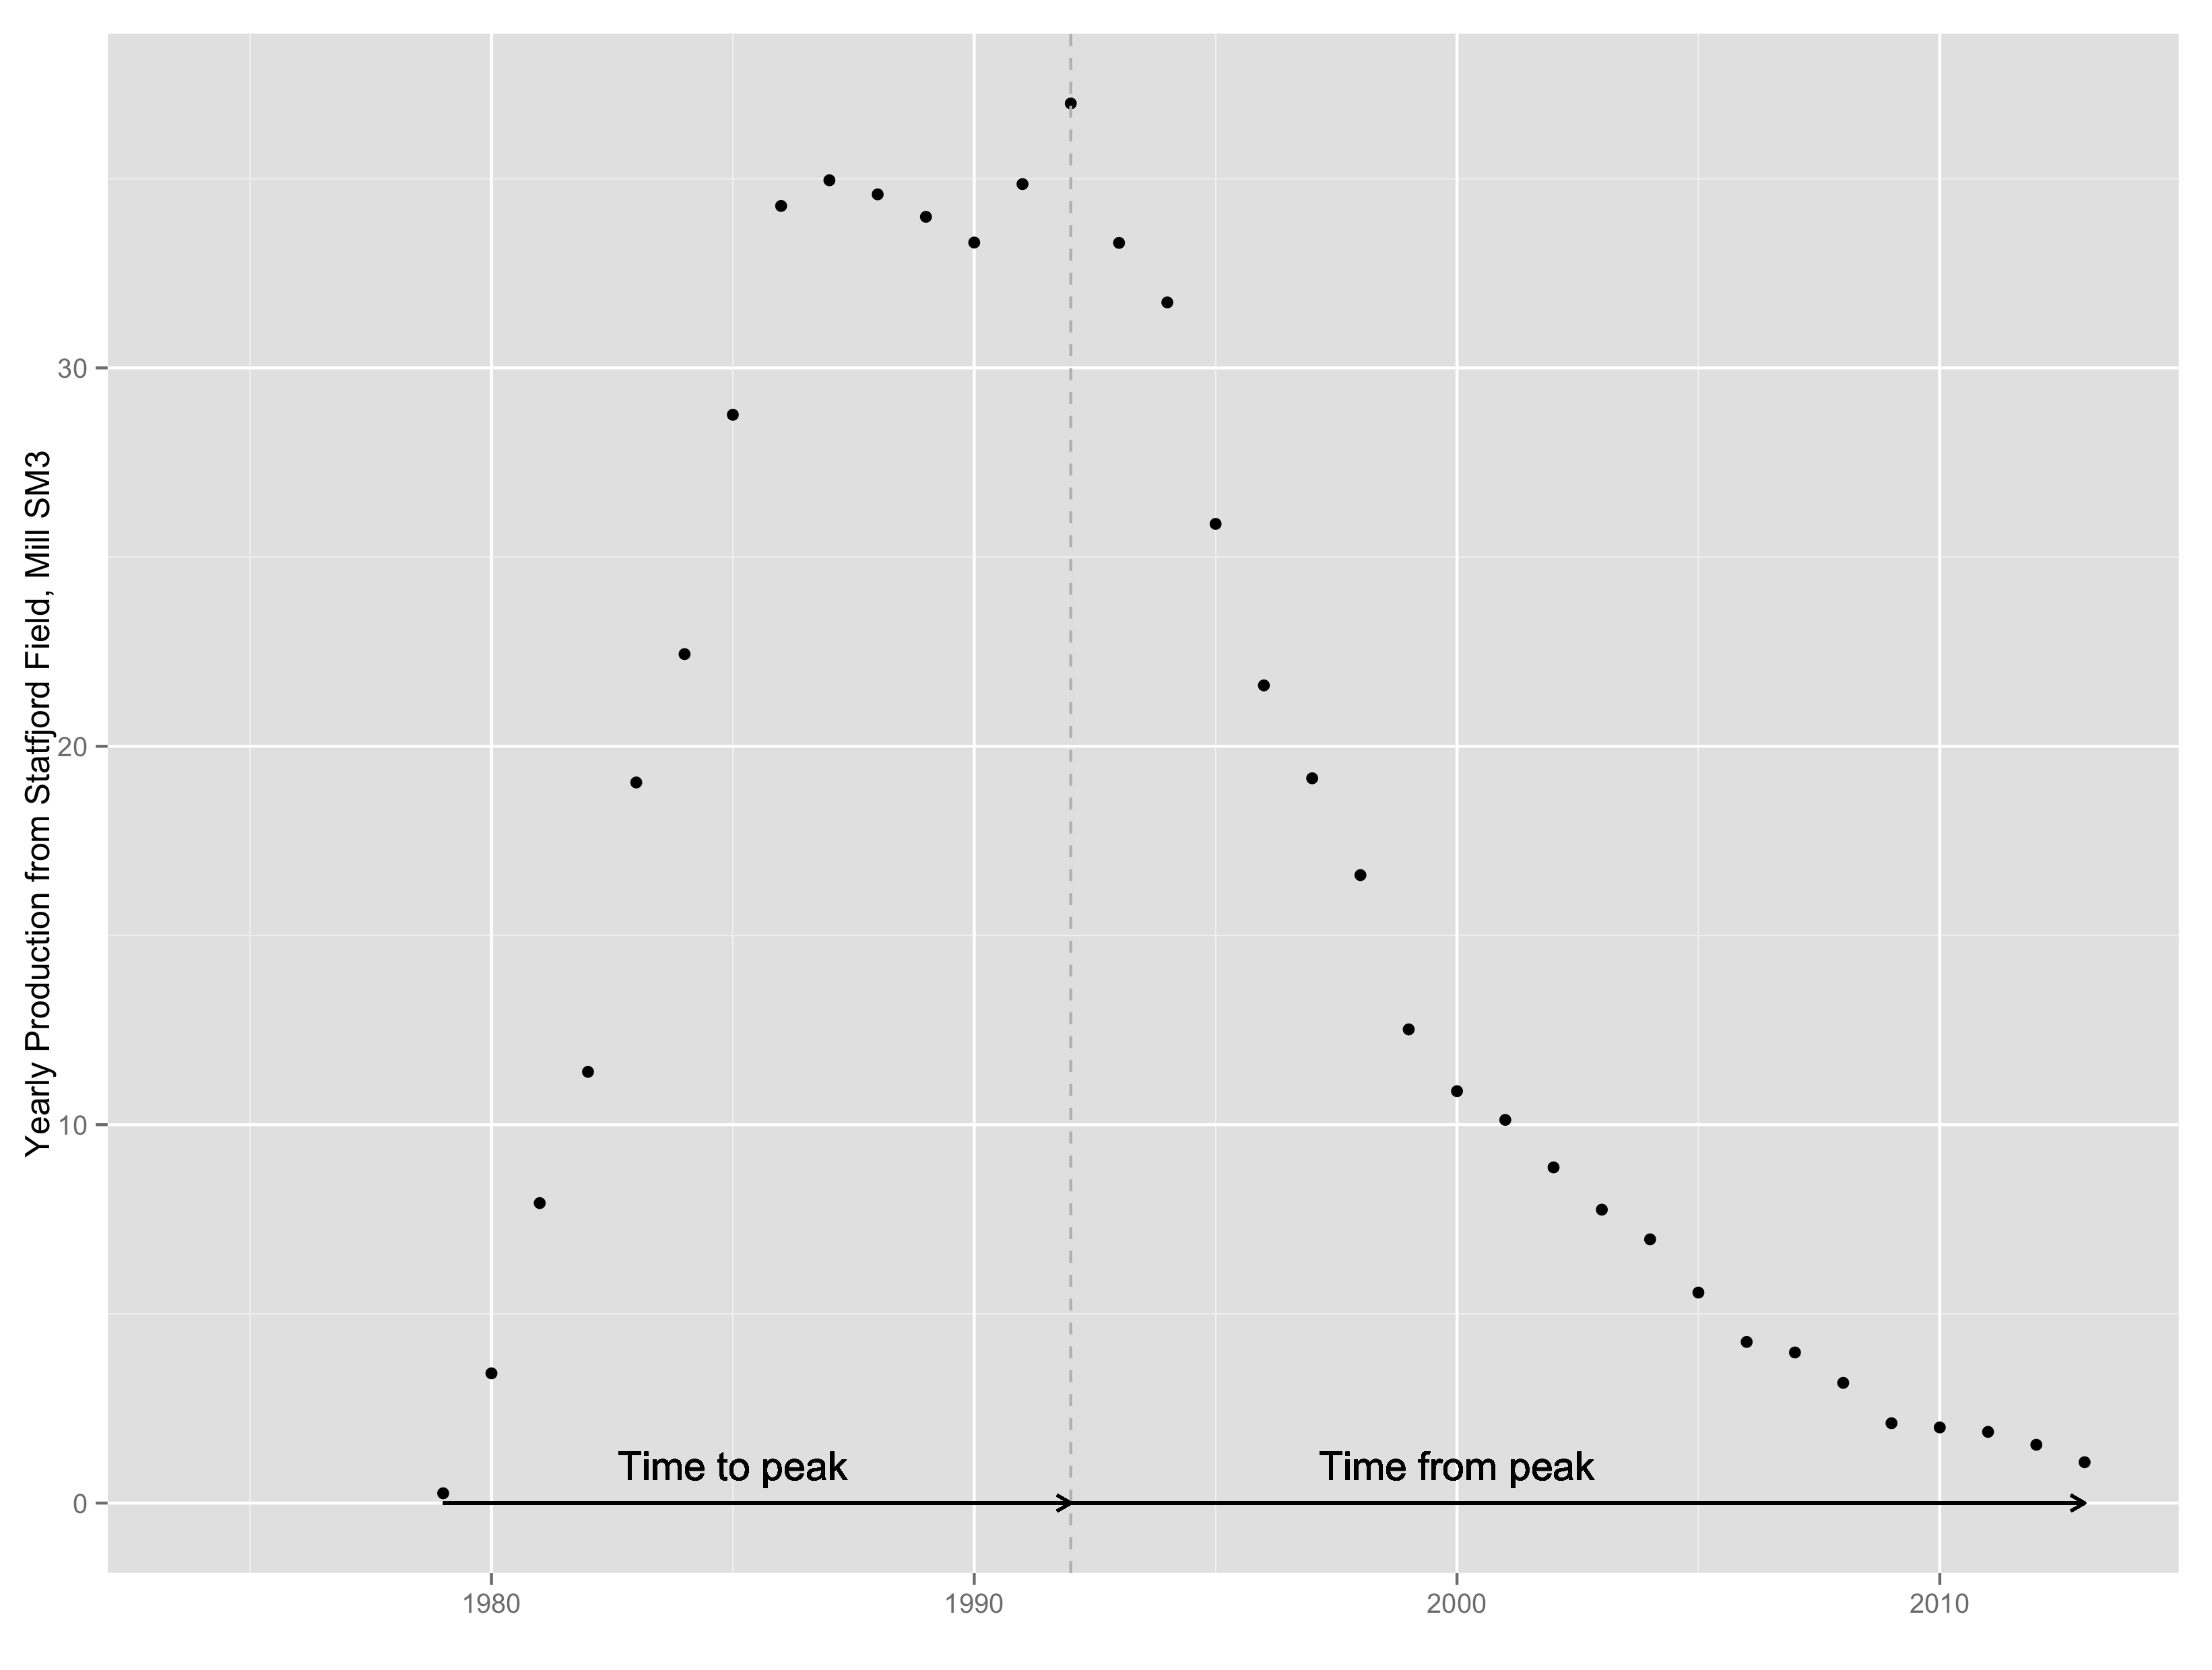
\includegraphics[width=.8\textwidth]{statfjord_dem.png}
\caption{}
\label{statfjord_dem}
\end{figure}

Figure \ref{glm_dirty_box} shows the estimates of the coefficients on the oil price and its lags \footnote{The dots on the figure represent 1000 simulations of the estimated coefficient based on the estimated standard error and point estimate from the model}.  The lags are not estimated to have an effect significantly different from zero. However a literal interpretation of the coefficients would indicate that a 10-dollar increase in the oil price would lead to a lowering of field production of around 2\%.

\begin{figure}
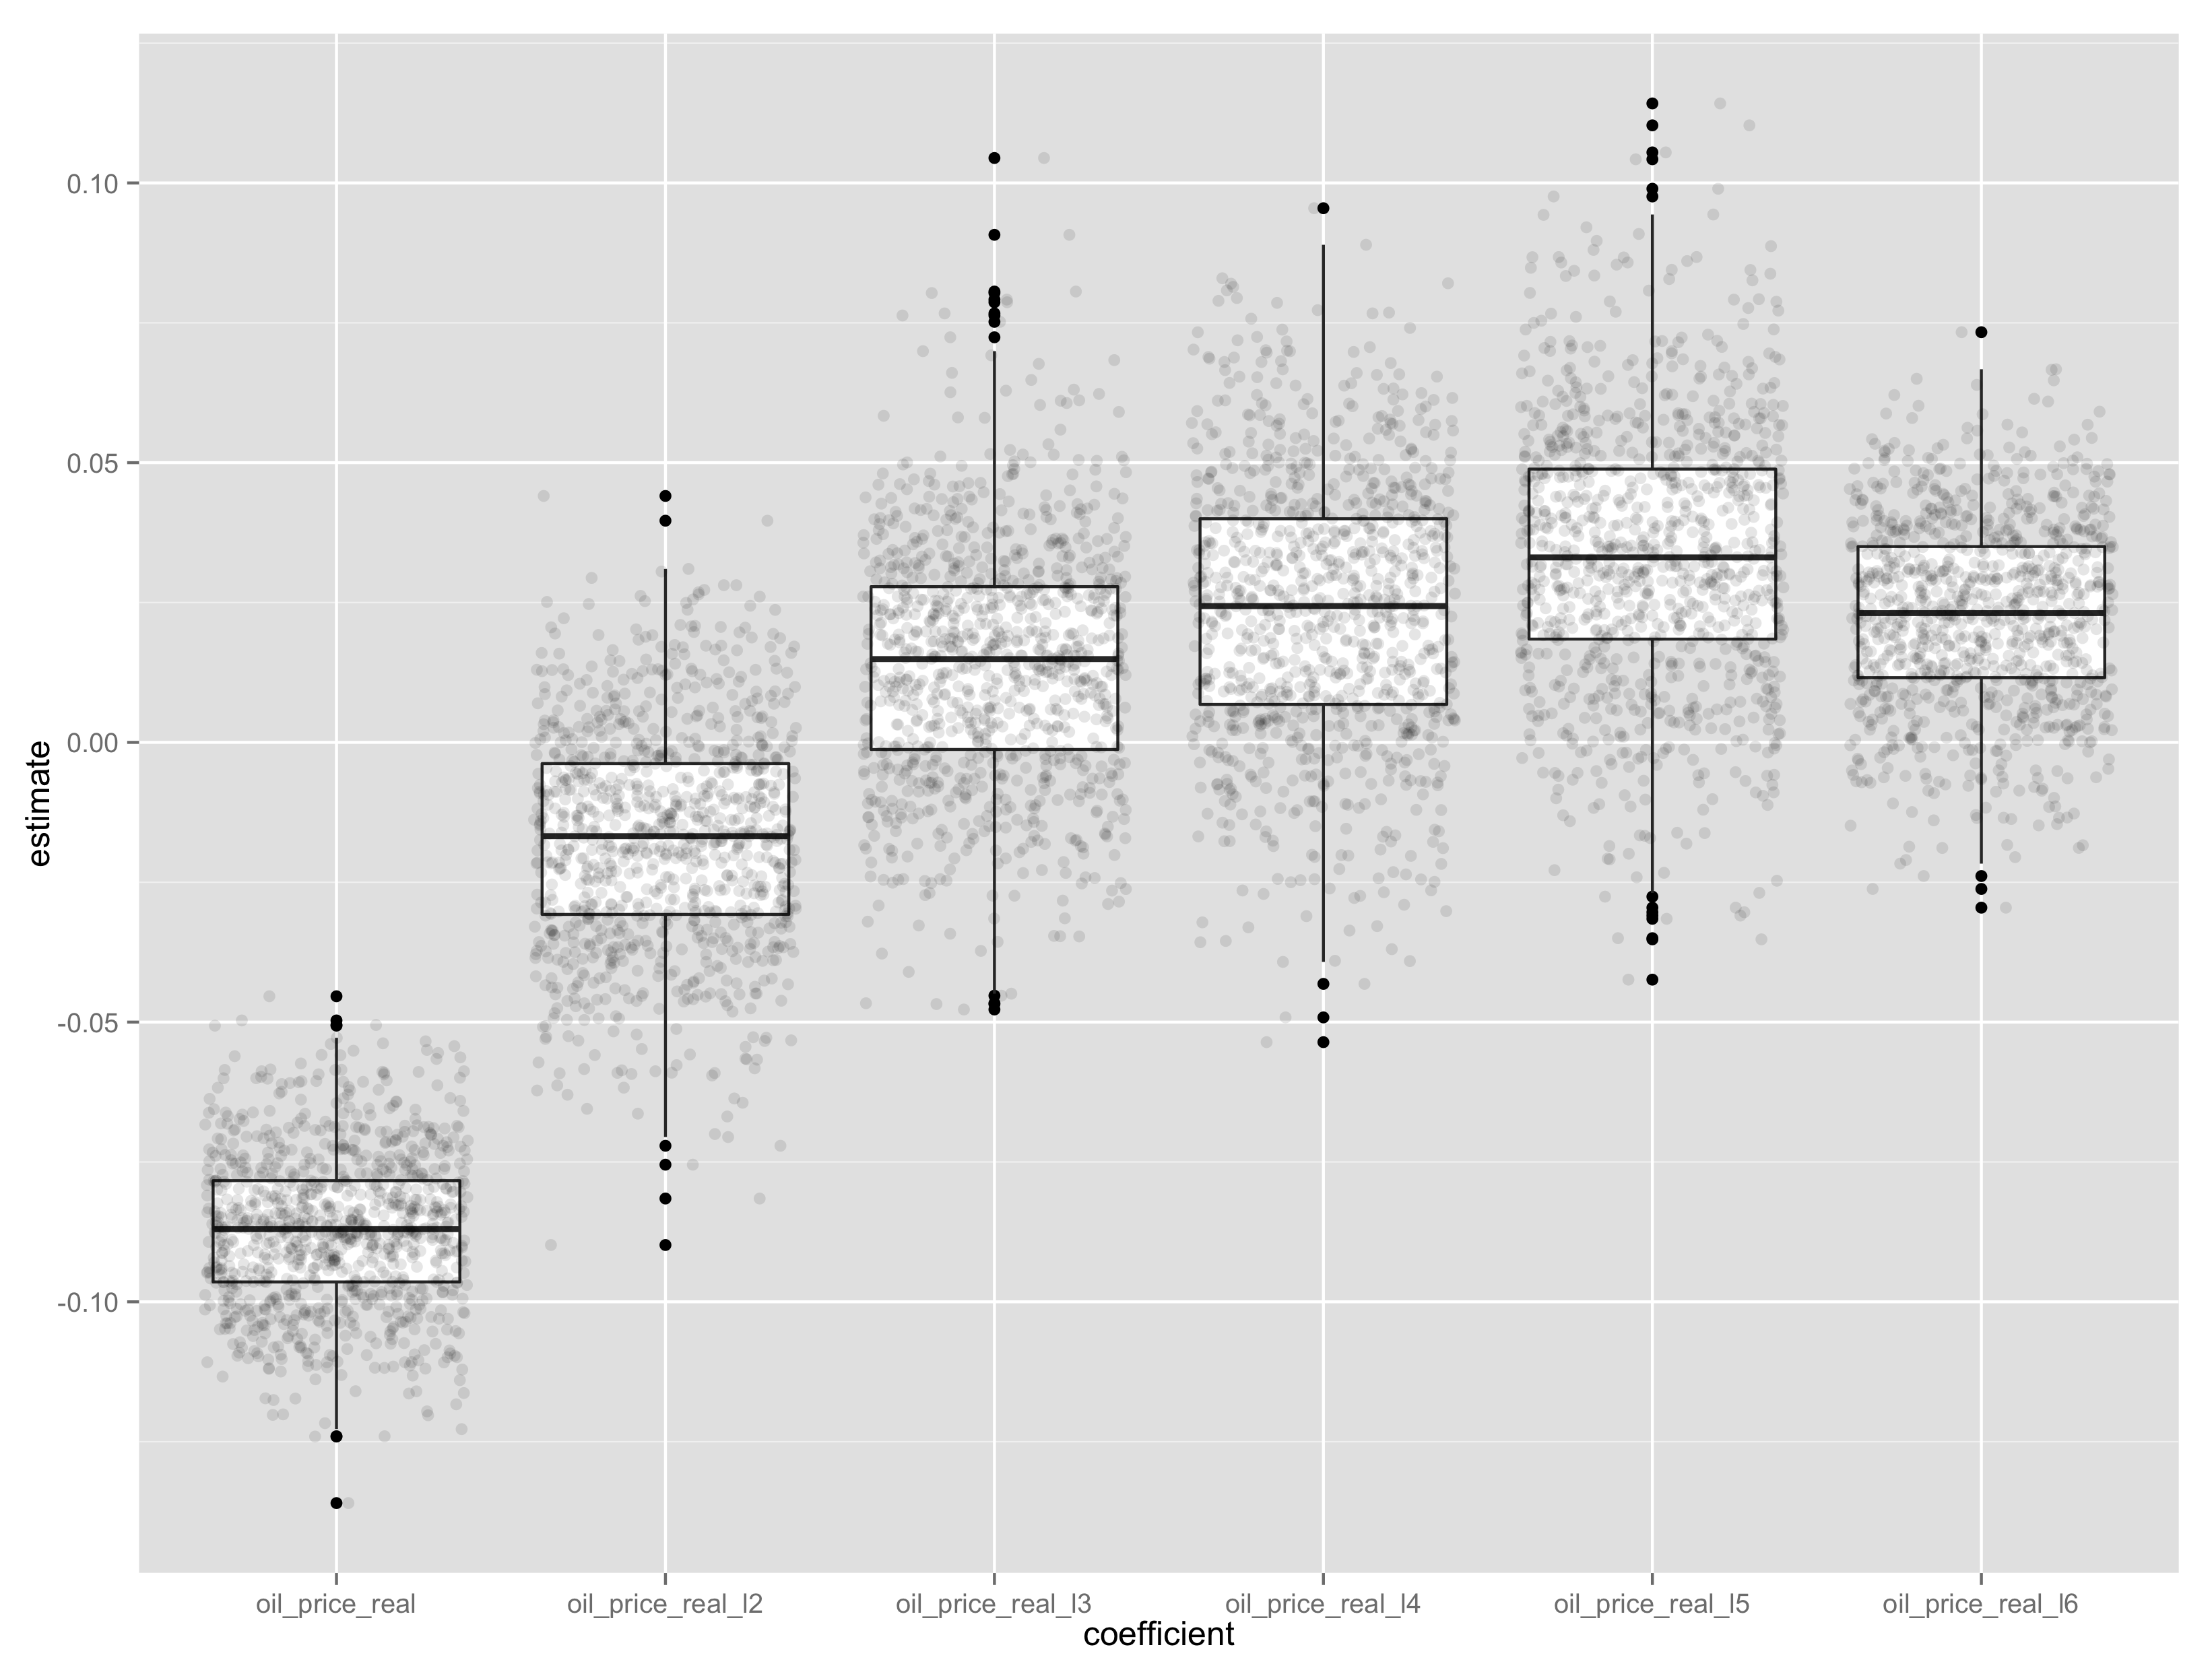
\includegraphics[width=.8\textwidth]{glm_dirty_box.png}
\caption{}
\label{glm_dirty_box}
\end{figure}

The estimates are of course heavily biased downwards due to the spurious correlation between the field production profiles and the autocorrelated time series of Brent oil prices.  The parametric representation is not flexible enough to control for the production profile of the fields.  Instead, a more flexible estimation of the production profile is needed. 

Instead of attempting to estimate the shape of the production profiles of the fields by estimating parameters on linear terms I estimate a non-parametric function for the production profile.  As an illustration, consider the production profile of a single field.  The simplest possible model would then have the form of equation \ref{simp_eqn}. 

\begin{equation}
Production_{t}=f(time) + \epsilon
	\label{simp_eqn}
\end{equation}

Again considering the production profile for the Statfjord field, a smoothed function might look like the black line in figure \ref{statfjord_gam}.   

\begin{figure}
	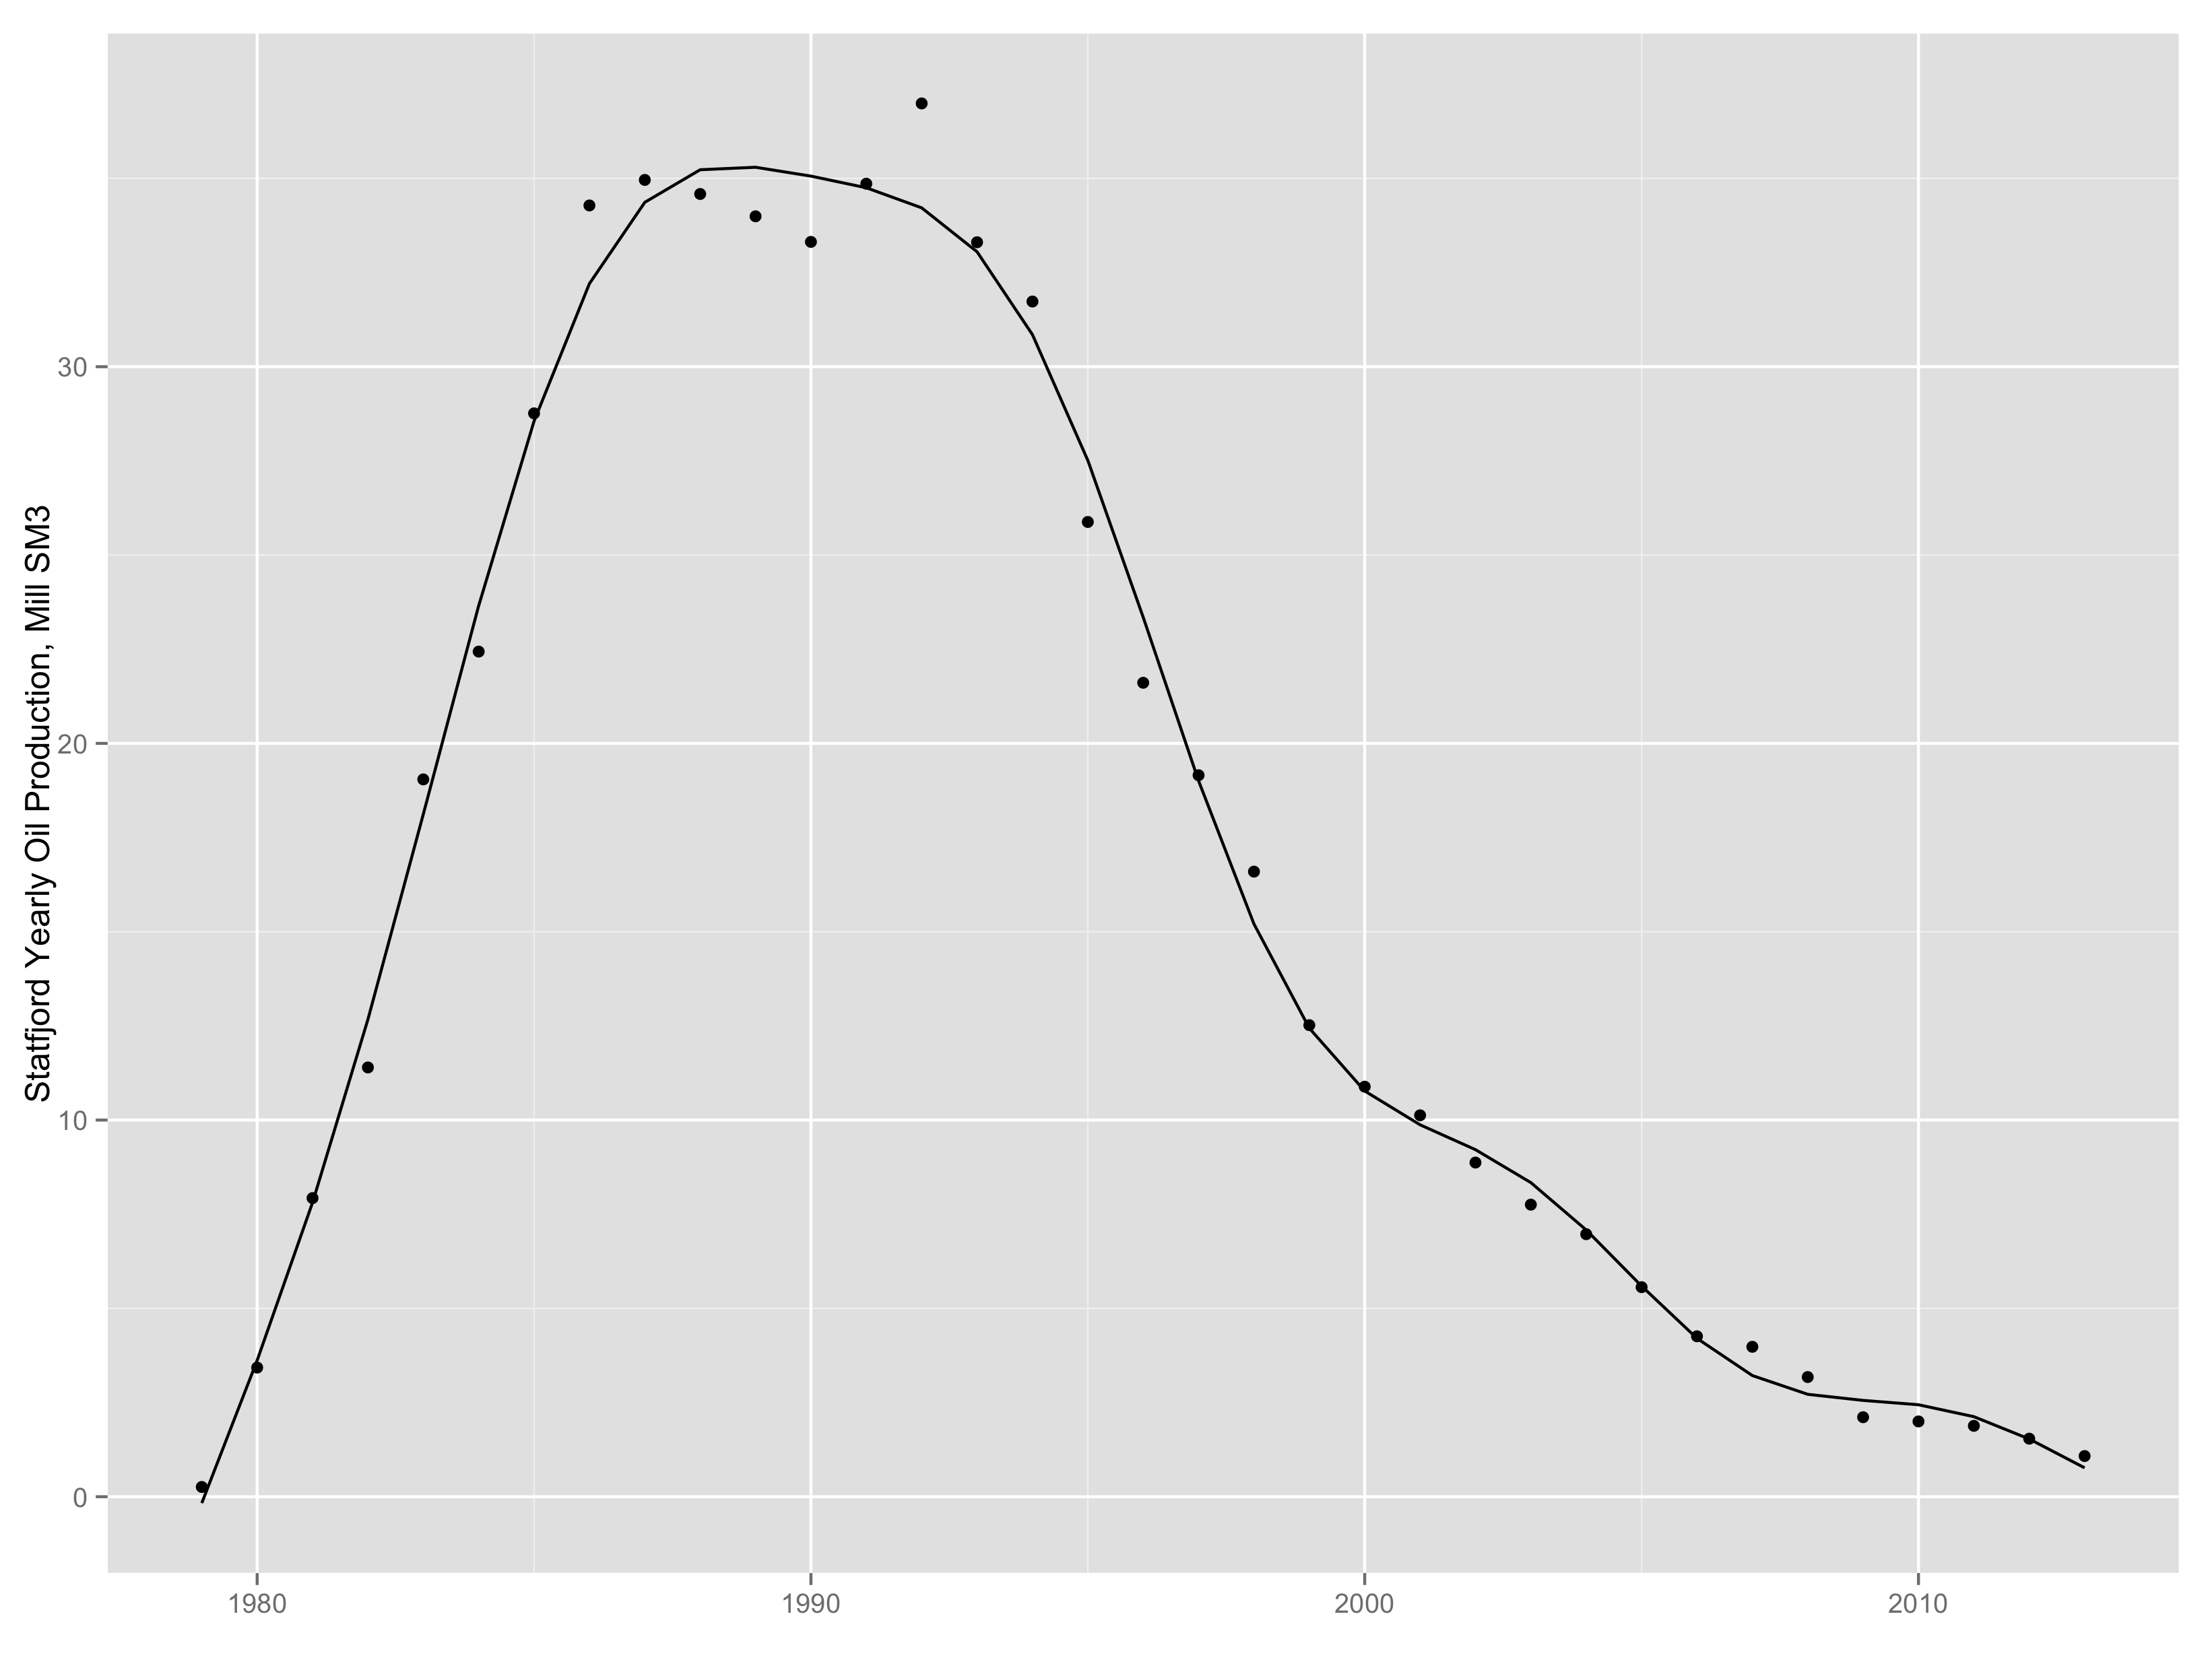
\includegraphics[width=.8\textwidth]{statfjord_gam.png}
	\caption{}
	\label{statfjord_gam}
\end{figure}

In principle any number of well-behaved smoothers could be used to estimate the function, for example a Loess or a kernel smoother.  In practice regression splines are most commonly used.  With a regression spline the data points for the function to be estimated is broken into bins.  For each bin of data a local linear regression is estimated.  For functions of one variable, a cubic parameterization is often used.  These regressions are then essentially tied together at what are called “knots” and the smoothness of the overall function is controlled by a penalty function that consists of the second derivative of estimated function.

The advantage to using splines over other smoothing methods is that it can be represented in a linear form.  Thus estimation of the model can be done by standard and efficient matrix algebra algorithms.  Variants of an iterative back-fitting least square procedure is the most common fitting procedure.  For further details I refer to the discussion in \citet{hastie_generalized_1990} and \citet{wood_generalized_2006}.  The latter is a particularly useful reference for implementing generalized additive models in R.  As a general note, this paper is not meant as a methodological piece.  The methods used here, while still not common in economics, are mature, developed and commonly used in Statistics as well as by other empirical researchers.

Of course, I do not want to estimate smoothed curves individually for each field.  While this would provide a good overall fit to the full data set, it would not be particularly information.  Instead I want to estimate a general shape of the production profile for all fields and then use the remaining variation in the data to see what effect price has.  My model can be written as in equations \ref{gam_price_eqn}.

\begin{equation}
\begin{split}
	Log(Production_{i,t})&=f(time\_to\_peak_{i,t}, total\_recoverable\_oil_i) \\
	& \quad + f(peak\_to\_end_{i,t}, total\_recoverable\_oil_i) \\
	& \quad + \beta_1 oil\_price + \beta_2 oil\_price\_l1 + ... +  \epsilon
\end{split}
\label{gam_price_eqn}
\end{equation}

In this model I am estimating the parameters and functions from all fields $i$. As in the parametric model presented earlier, the left-hand-side variable is yearly oil production for field $i$. Also like the parametric model I split the production-time component element in two -up to and after the peak in production.  While a shape for the entire production profile could be estimated with one smoothed function, splitting it up into two allowed for more flexibility and better overall fit of the model as estimated by deviance score and the related estimated degrees of freedom of the model.  

 I also allow the smoothed functions to vary with the total size of the field as measured by the estimated total recoverable oil since the shape of the production profile tends to vary substantially by field size.  Inspection of a selection of fields, such as shown in figure \ref{field_inspection}, shows that smaller fields tend to reach their peak quickly while larger fields, which need to be built up in order to reach their full production, take more time.   Such a two-dimensional function can not be estimated by a traditional cubic regression spline.  Instead what a thin-plate spline \citep[p.150]{wood_generalized_2006} is used to estimate the smoothed functions.

\begin{figure}
	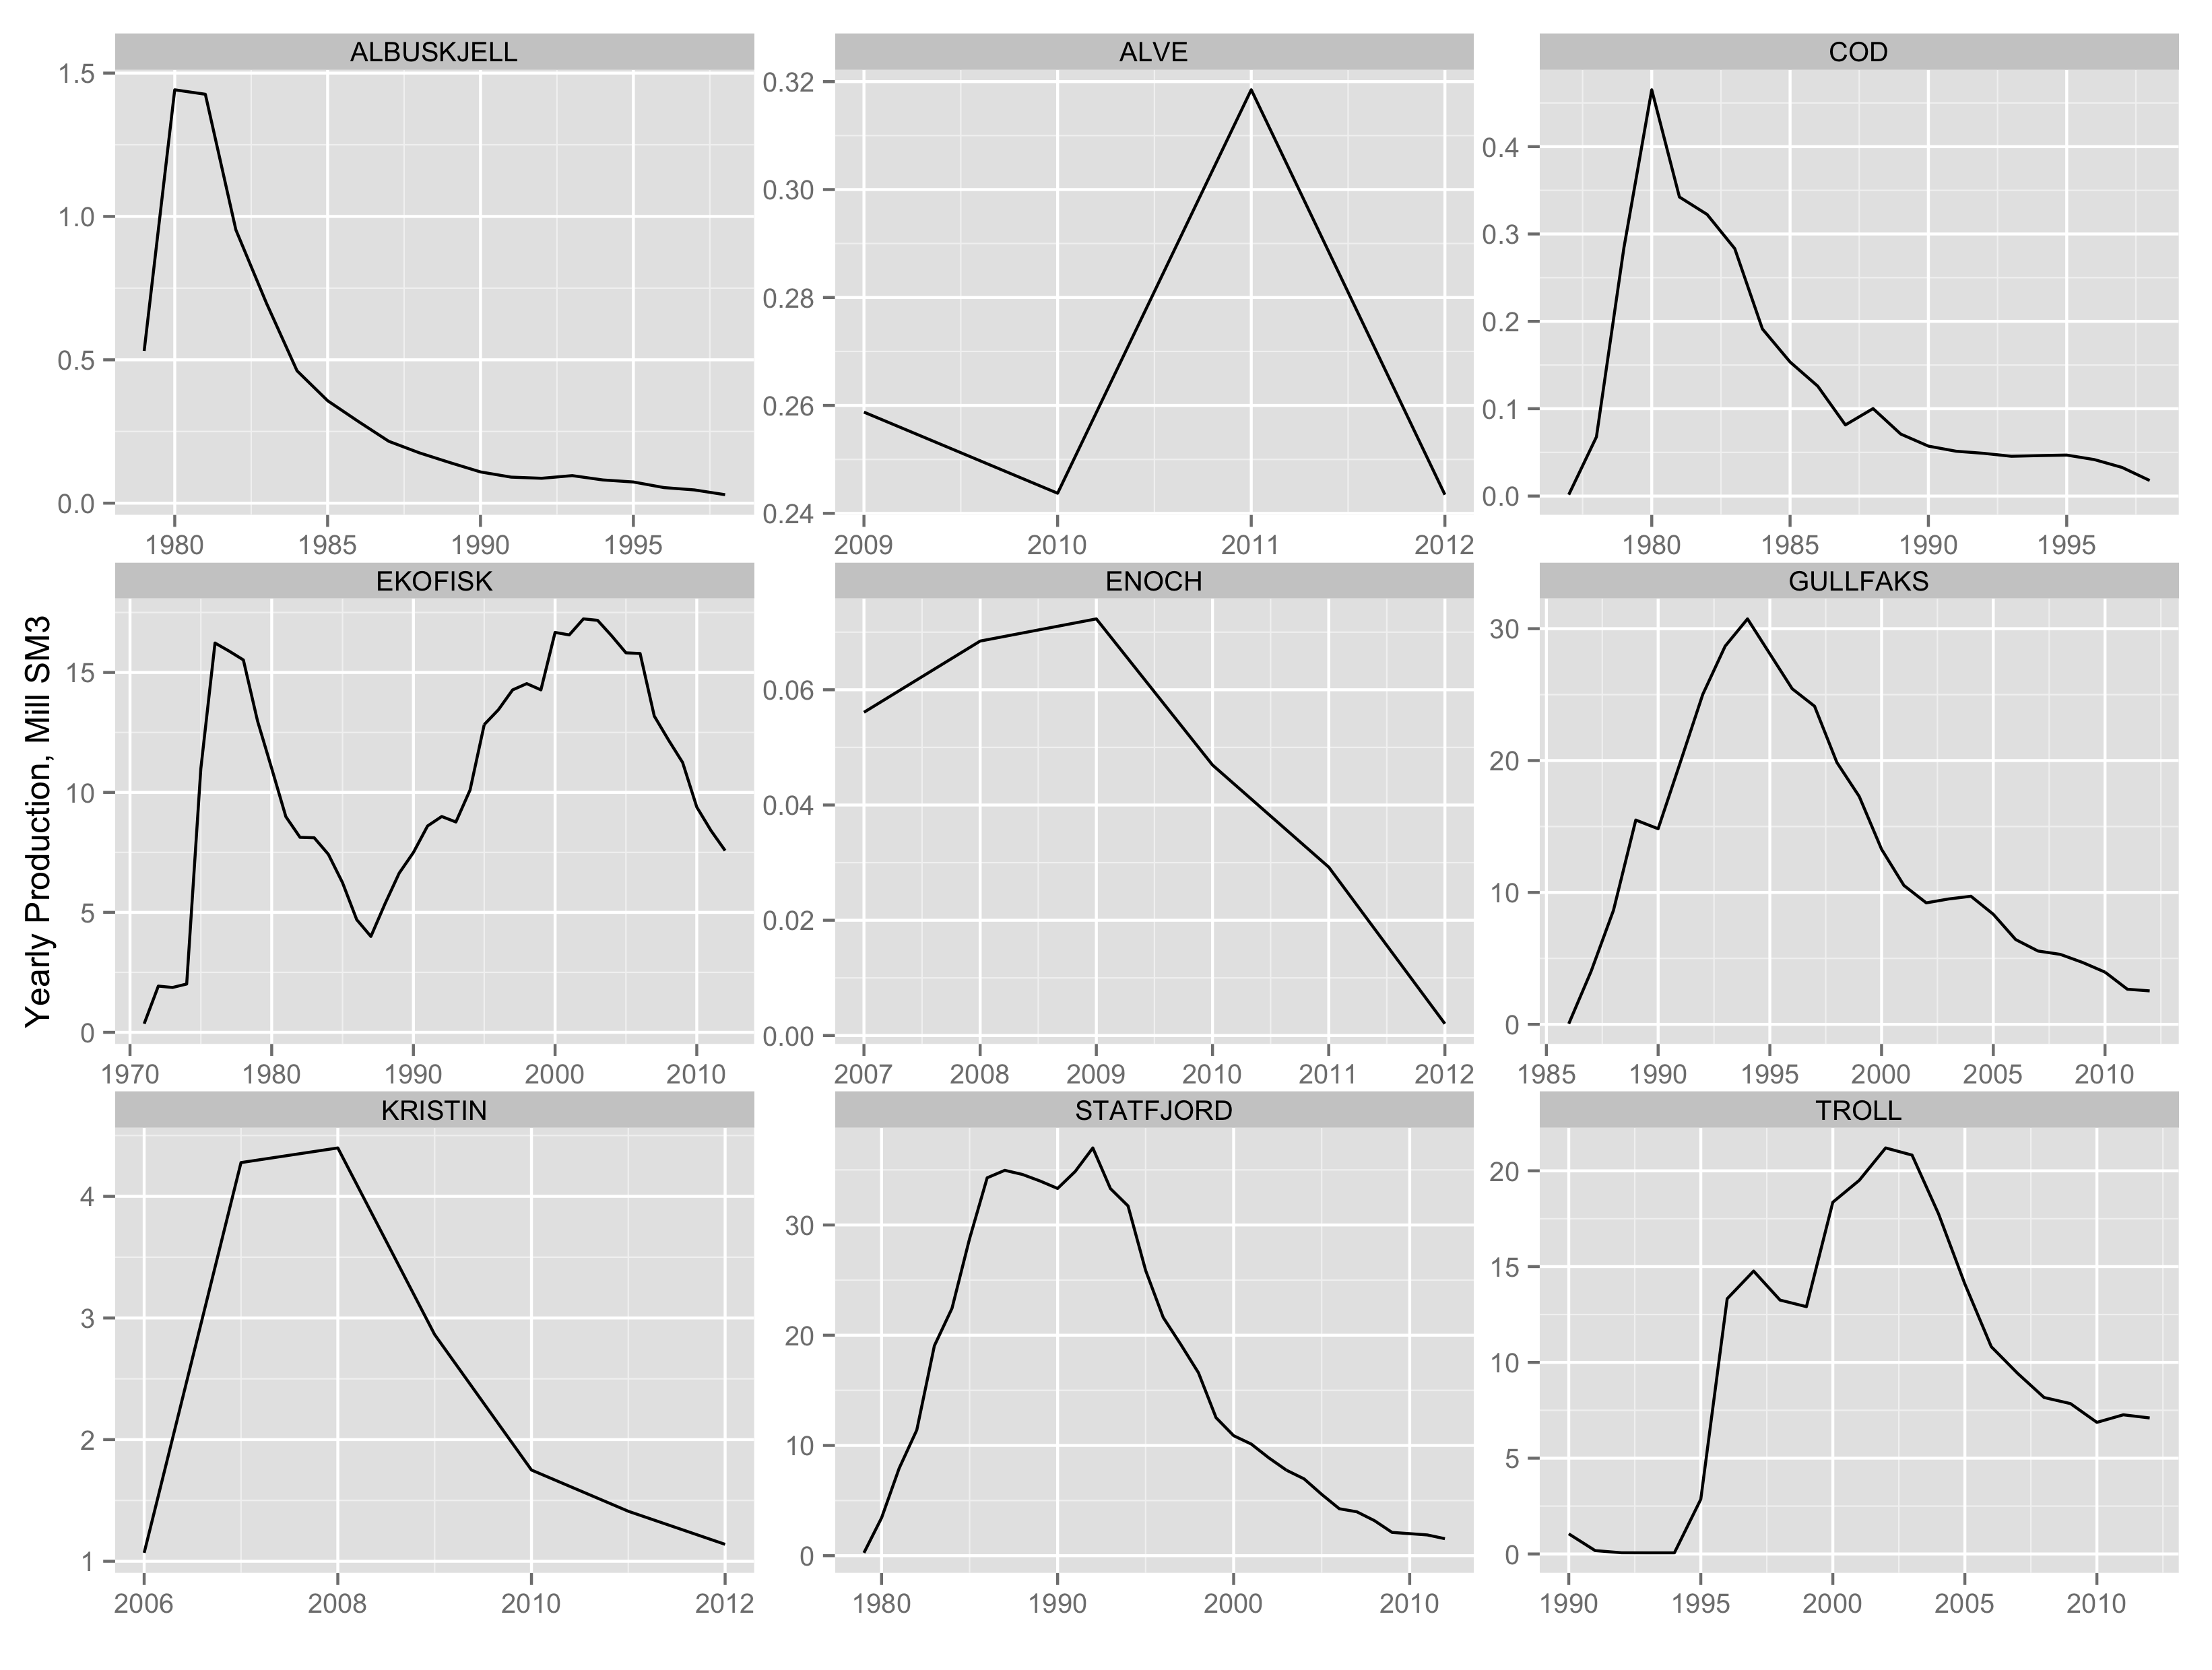
\includegraphics[width=.8\textwidth]{field_inspection.png}
	\caption{}
	\label{field_inspection}
\end{figure}

Even with a smoothed function that is allowed to vary by field-size, a substantially better fit could be obtained by splitting the estimation into small and large fields, this time measured by max production year.  The improvement in fit can be seen by inspecting the fitted values of the models as in figure \ref{bench_vs_split}. The split estimation provides a particularly better fit for smaller and mid-sized fields.

\begin{figure}
	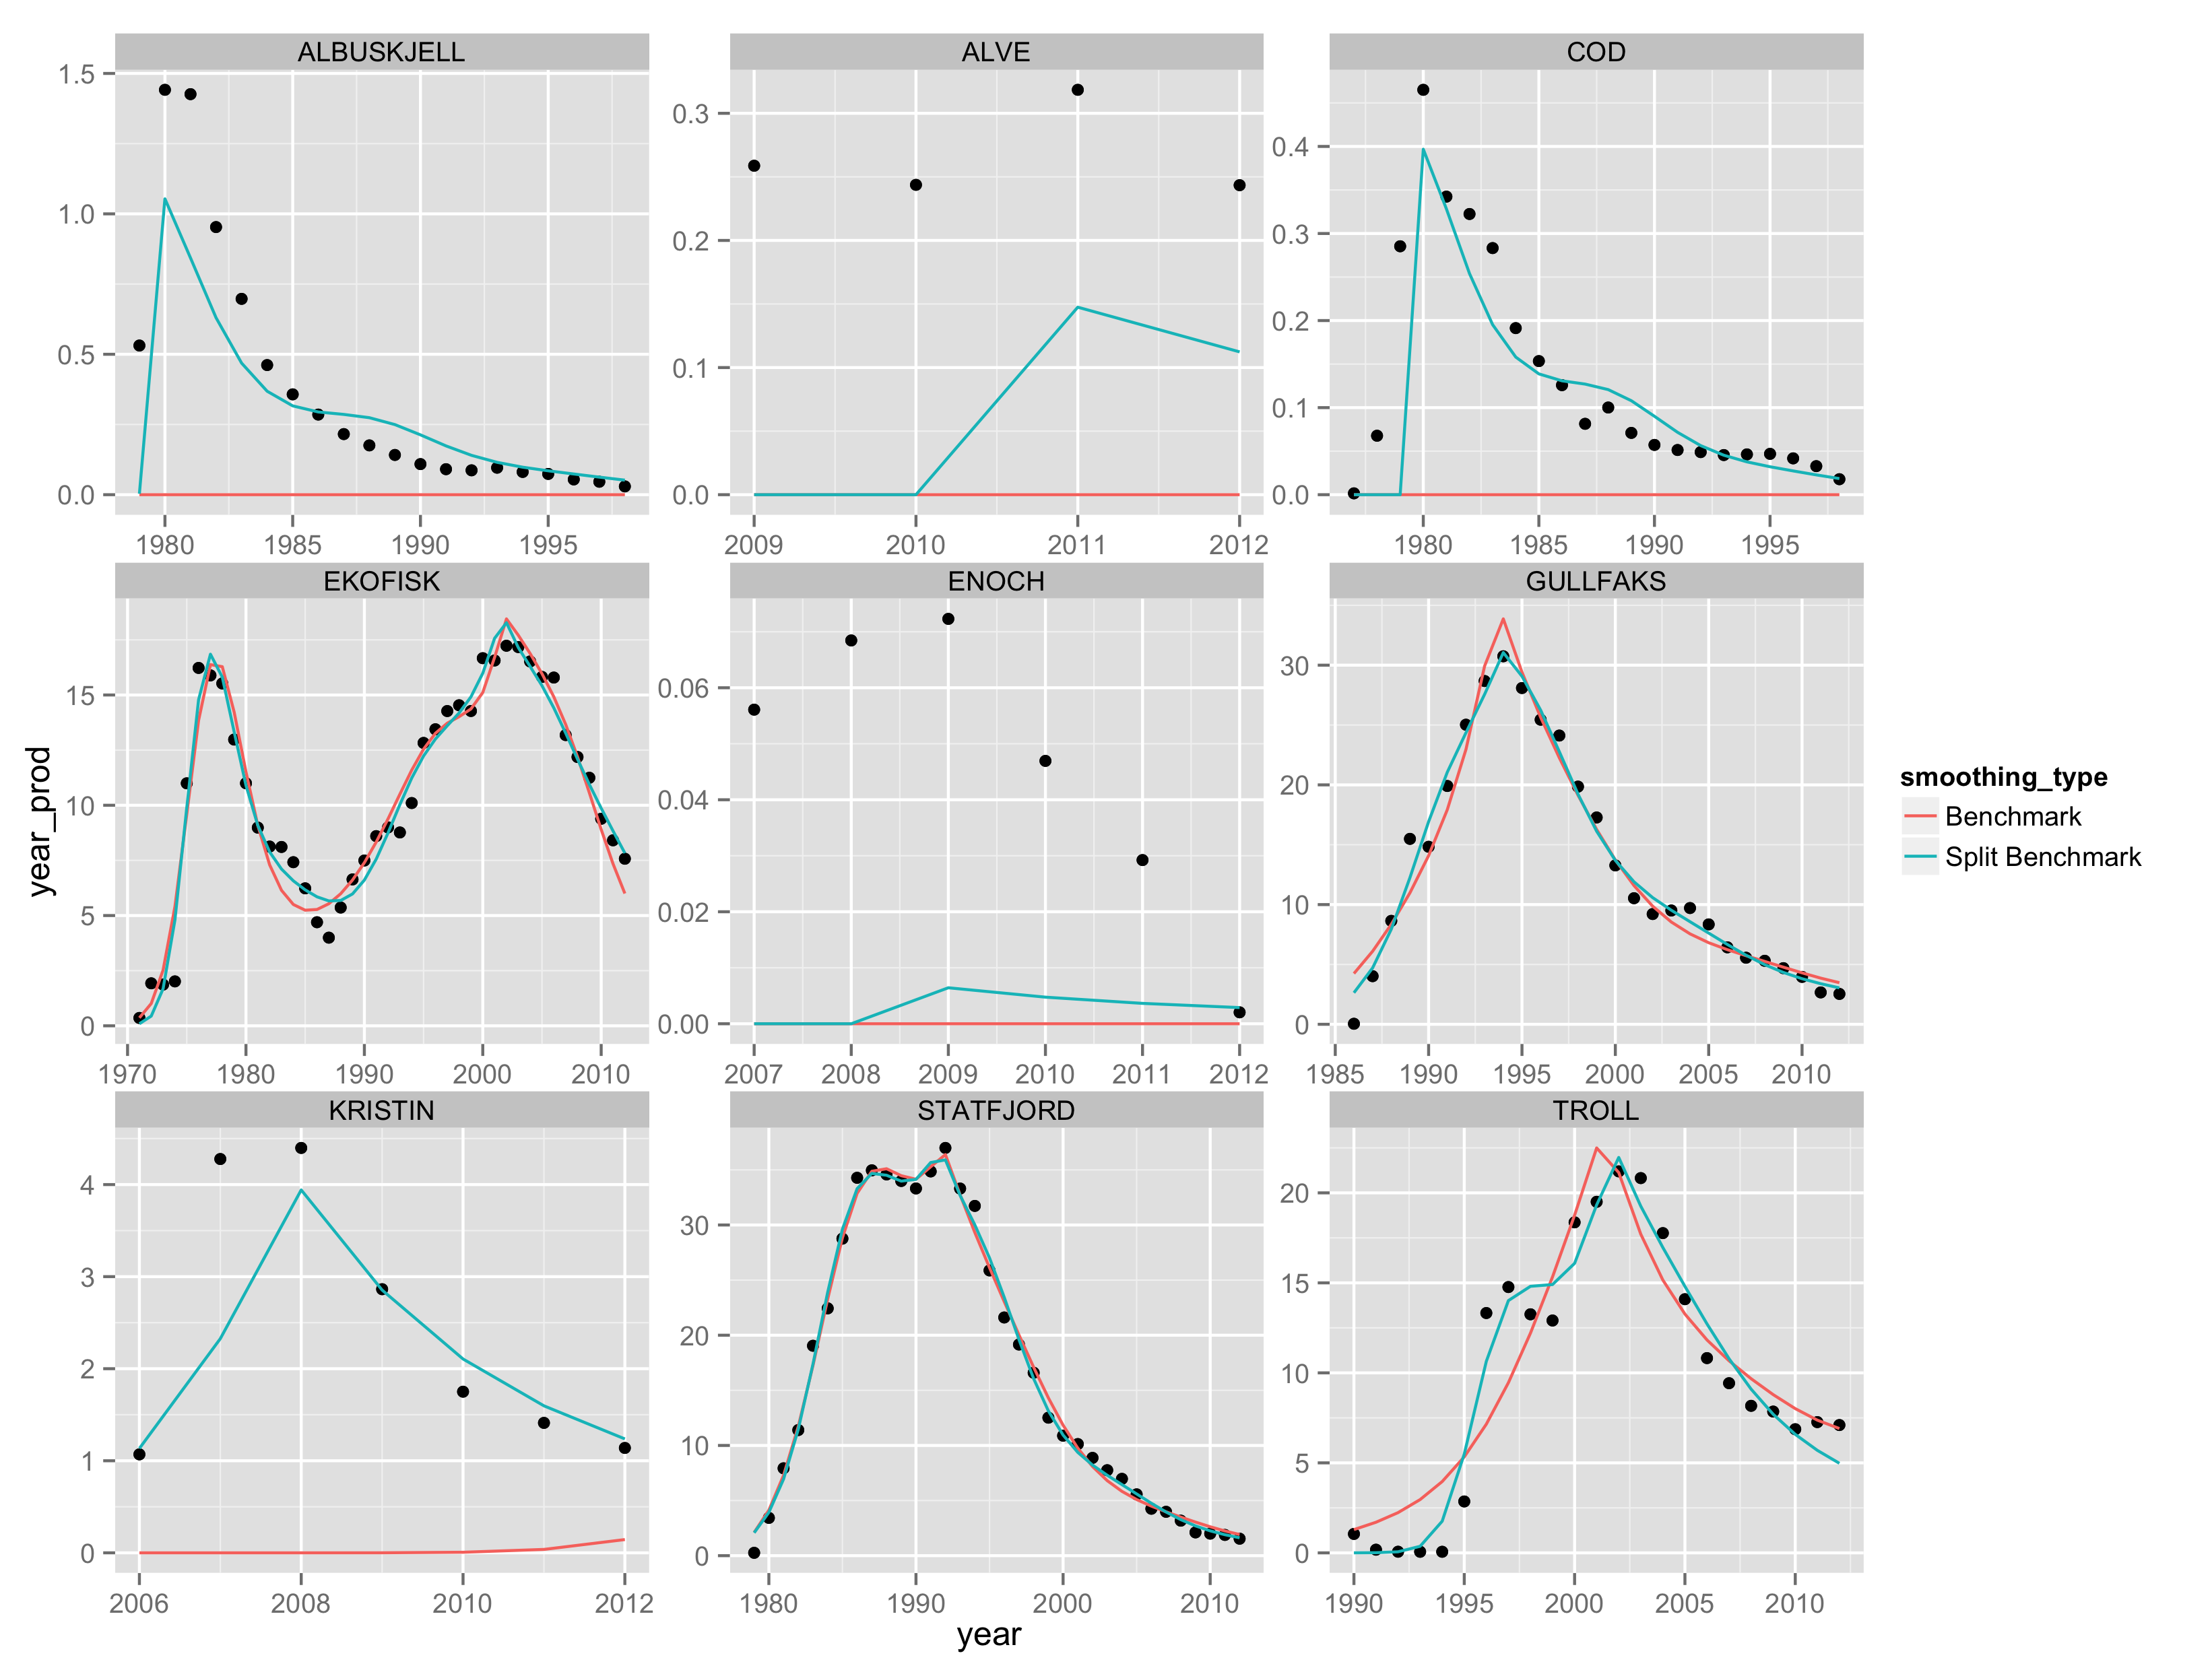
\includegraphics[width=.8\textwidth]{bench_vs_split.png}
	\caption{}
	\label{bench_vs_split}
\end{figure}

\section{The Effect of Oil Price on Field Production}

The variables of interest is of the course the oil price, which I include as a linear parametric term in the model.  I also include six lags of the oil price variable in the model, again as linear parametric terms.  The idea of including both a concurrent oil price term as well as lags is that a change in price could conceivably have two effects on oil production in a field.  First, the field operator could be operating on the basis of some short-term extraction rule - choosing to pump out less at times of lower prices so that they could pump out more at periods of high prices.  

Alternatively, a change of oil prices can be seen as a lifting of a production constraint.  A higher oil price means that is worthwhile to invest more in production, increasing the current rate of production and potentially leading to an overall higher extraction rate.  

The estimates of the parametric oil price terms are shown in figure \ref{gam_price_dirty_box}.  What is shown is a box plot centered around the point estimate of each coefficient.  The box can be interpreted as a 50 percent confidence interval while the lines can be interpreted as a 95% confidence interval.  Estimates for fields with a maximum yearly production of over and under 8 million SM3 are shown.  

\begin{figure}
	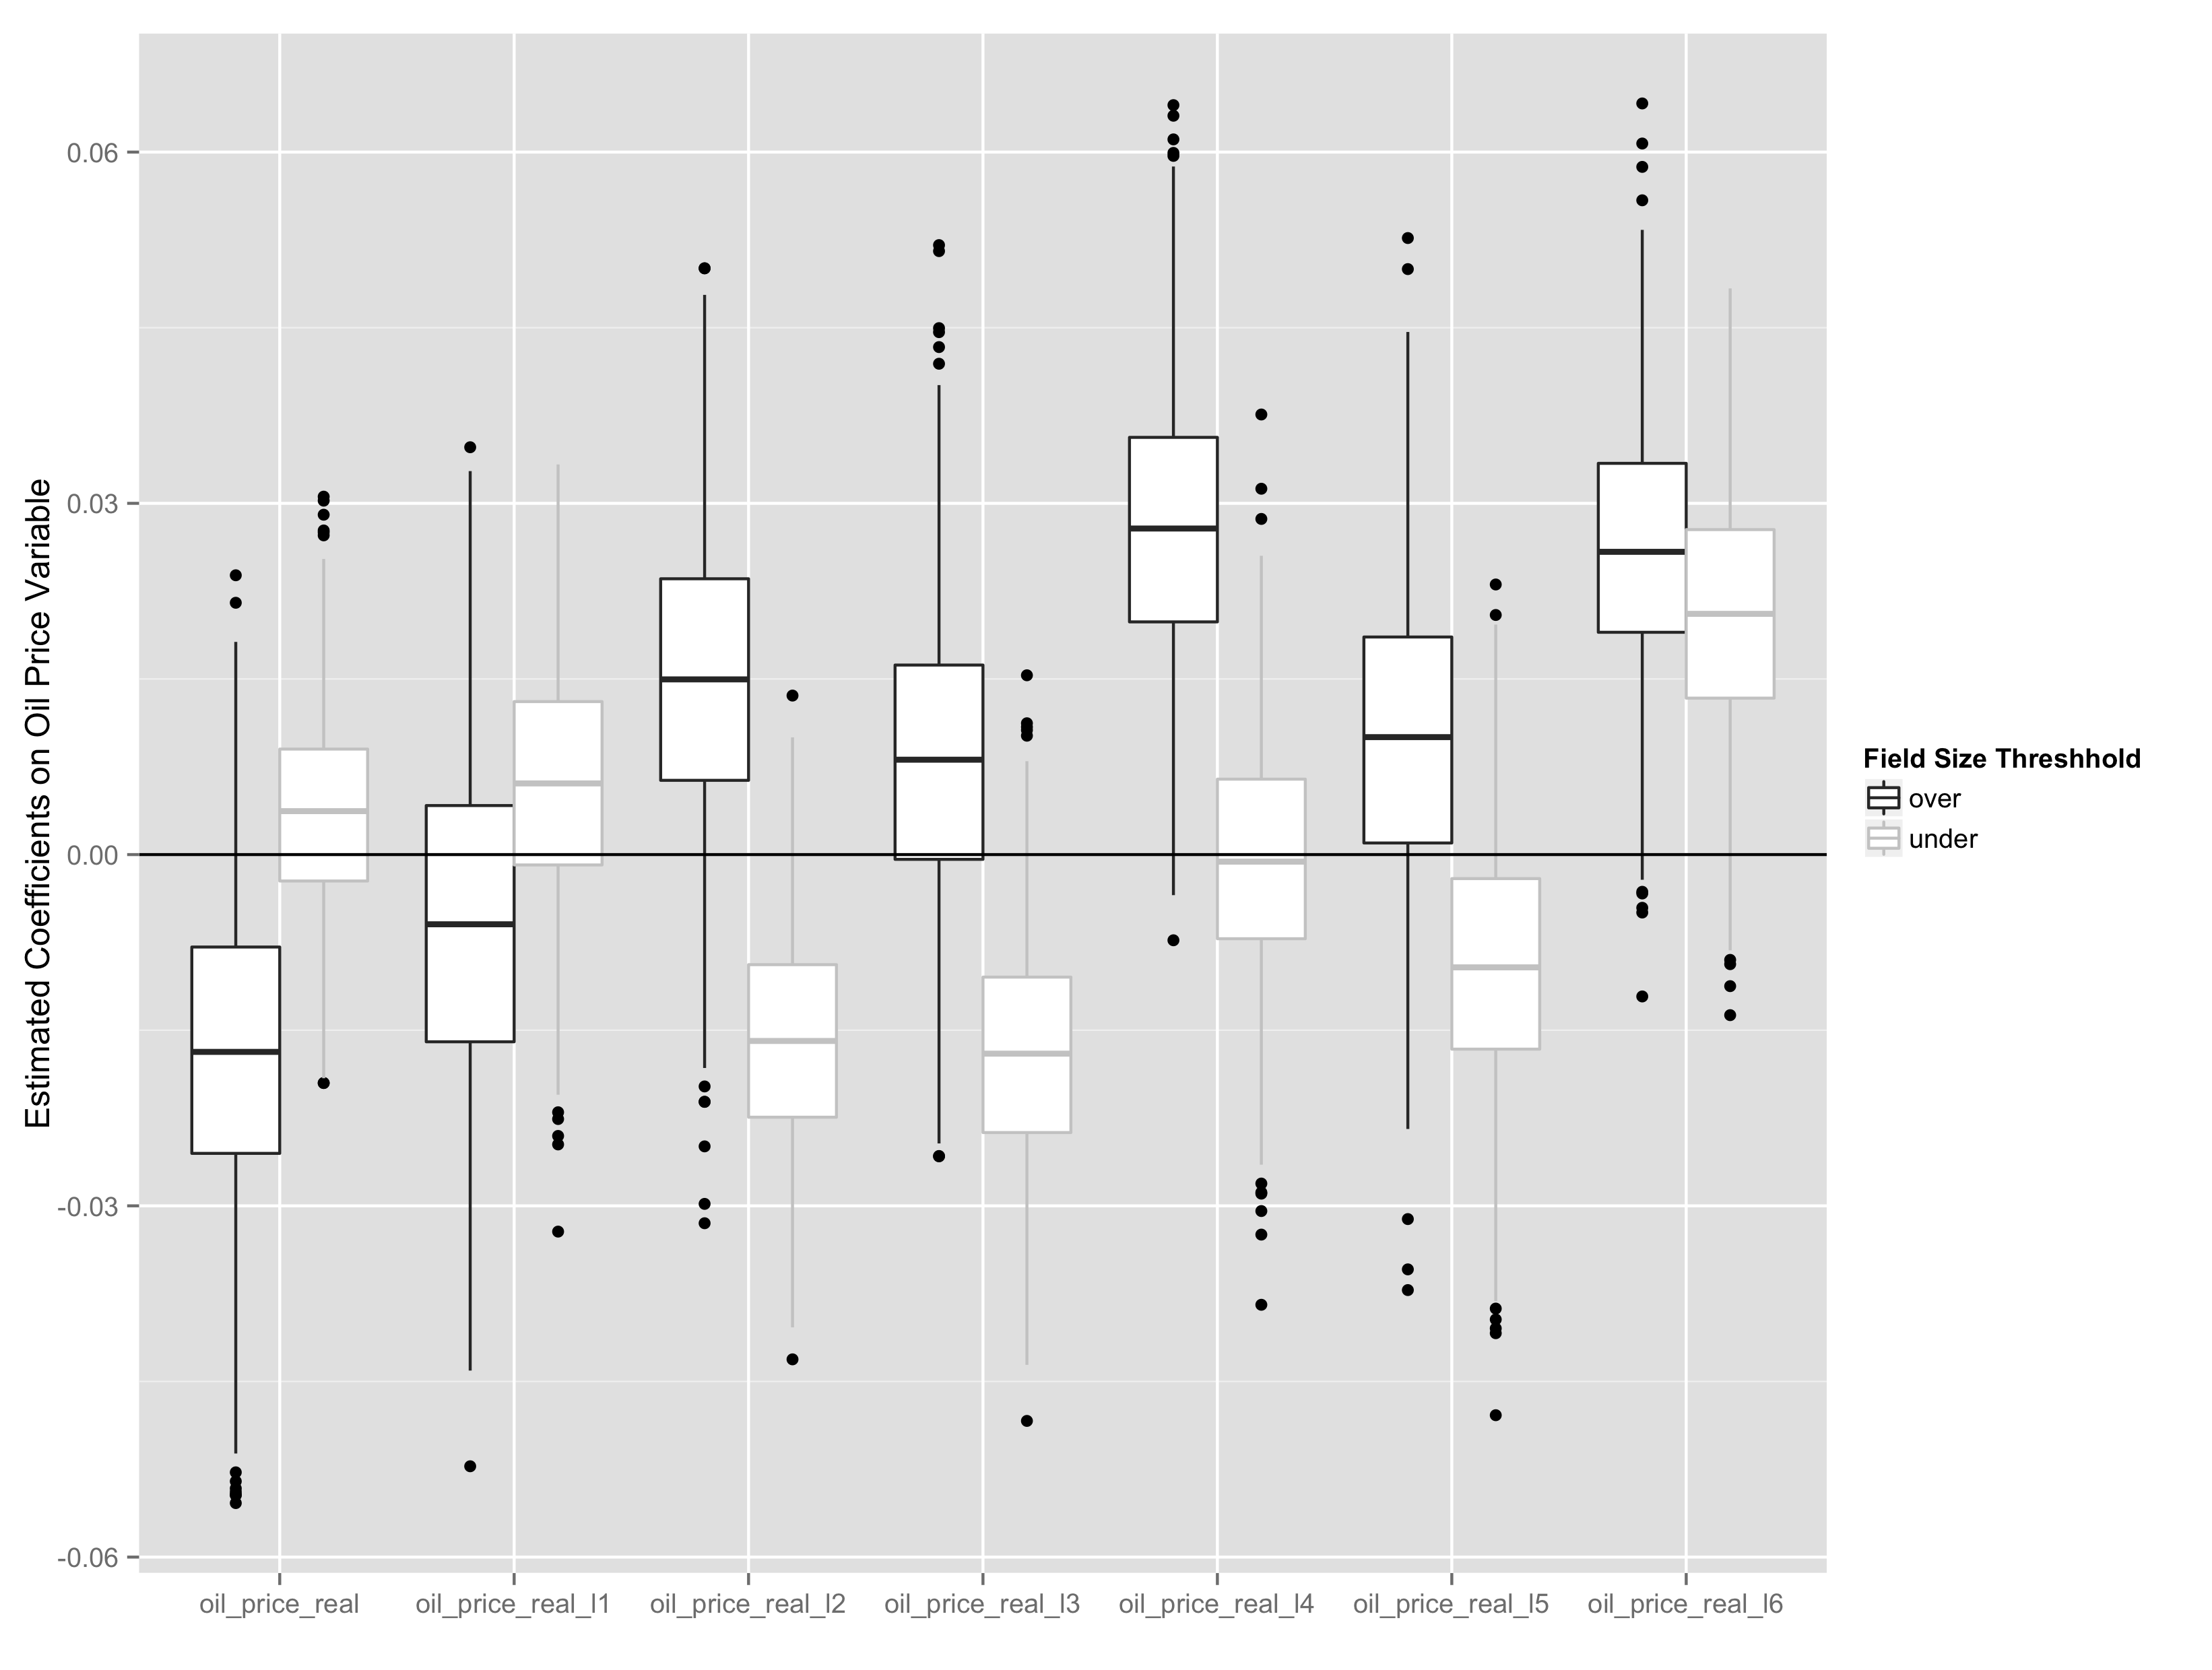
\includegraphics[width=.8\textwidth]{gam_price_dirty_box.png}
	\caption{}
	\label{gam_price_dirty_box}
\end{figure}

The estimated coefficients for the concurrent and first three lags of the oil price are not estimated to be significantly different than zero.  For large fields a modest effect at the fourth and sixth lags are estimated while for small fields an effect is estimated only at the sixth lags. The magnitude of these effects is in the neighborhood of a 2% increase in production for a 10 dollar increase in the oil price.  

As can also be seen from the figure, these estimates are right on the margin of the traditional 95 percent confidence threshold.  However the estimates due make some intuitive sense.  Discussions with people in the industry about the results also supports their validness.  In general, operating an oil production rig and related infrastructure is an extremely expensive venture with high fixed costs.  In the challenging conditions of the North Sea, the expenses are multiplied.  Thus any short term benefit of strategically altering production in relation to movements in the oil price are dominated by the large costs of having excess capacity.  In other words, oil producers have a strong incentive to pump as much oil out at any given time given the existing production capacity.  

This may be because higher oil prices allow for more sophisticated and expensive extraction techniques that will increase the total extraction rate of a field - that is the fraction of oil from the field that can be profitably extracted.  This story is in line with a trend of increased total extraction estimates from the Norwegian continental shelf over the last 15 years of strongly rising oil prices \citep{npd}.  

Another potential motive is that higher oil prices leads companies to expand the production rate in the face of uncertain future oil prices.  While not strategic in the sense discussed earlier of having spare capacity ready and reacting to short-term price movements, it would mean companies are changing their level of investment in order to shift the production profile over time - a higher price induces companies to produce more relatively sooner thus leaving less in the ground for future production.  In reality, the motive is likely a combination of the above factors - an oil price induces investment in increased production capacity in order to both shift forward production as well as increase the overall extraction rate.  

In the above discussion, I have been implicitly giving the coefficients a causal interpretation, which deserves some discussion.  My main identifying assumption is that production on the field level can not cause significant changes in the oil price.  A stronger but still relevant assumption that may be necessary since fields production is correlated across fields is that total production from the Norwegian continental shelf does not effect oil price.  Both of these assumptions are likely satisfied.  Oil is a globally traded commodity and total Norwegian production accounts only for a small fraction of total production.  In 2013 Norwegian production made up only 2.3 percent of the world total.  A drastic change in production, on par with the halt in production that occurred in Libya in 2012, would have been required to have had any significant effect on world oil supply and in turn prices.  

One of the main implications of the interpretation that higher oil prices leads to increased extraction through increased capacity is that while the effect on production will be lagged, higher oil prices will have a more immediate effect on investments.  I test for this with the model as written in equation \ref{gam_invest_eqn}

\begin{equation}
\begin{split}
	Log(Investment_{i,t})&=f(time\_to\_peak_{i,t}, total\_recoverable\_oil_i) \\
	& \quad + f(peak\_to\_end_{i,t}, total\_recoverable\_oil_i) + oil_production_{i,t} \\
	& \quad + \beta_1 oil\_price + \beta_2 oil\_price\_l1 + ... +  \epsilon
\end{split}
\label{gam_invest_eqn}
\end{equation}

In the equation investment in each field $i$ at time $t$ is a function of the state of field development, as modeled by a non-parametric function of time to and from the peak as well as the total size of the field - as in the model of oil field production.  In addition I include a term for oil production in field $i$ at time $t$.  The coefficients of interest are again those on the oil price and its lags.  

The results for the estimation of the estimated coefficients on the oil price and its lags is shown in figure \ref{gam__price_invest_box}.  The coefficient on the concurrent oil price as well as the first two lags are all significantly positive, with coefficients that can be interpreted to mean that a 10 dollar increase in the oil price leads to between a 5 to 10 percent increase in oil field investment for the current and two subsequent years.  No significant effect can be estimated for subsequent lags however

\begin{figure}
	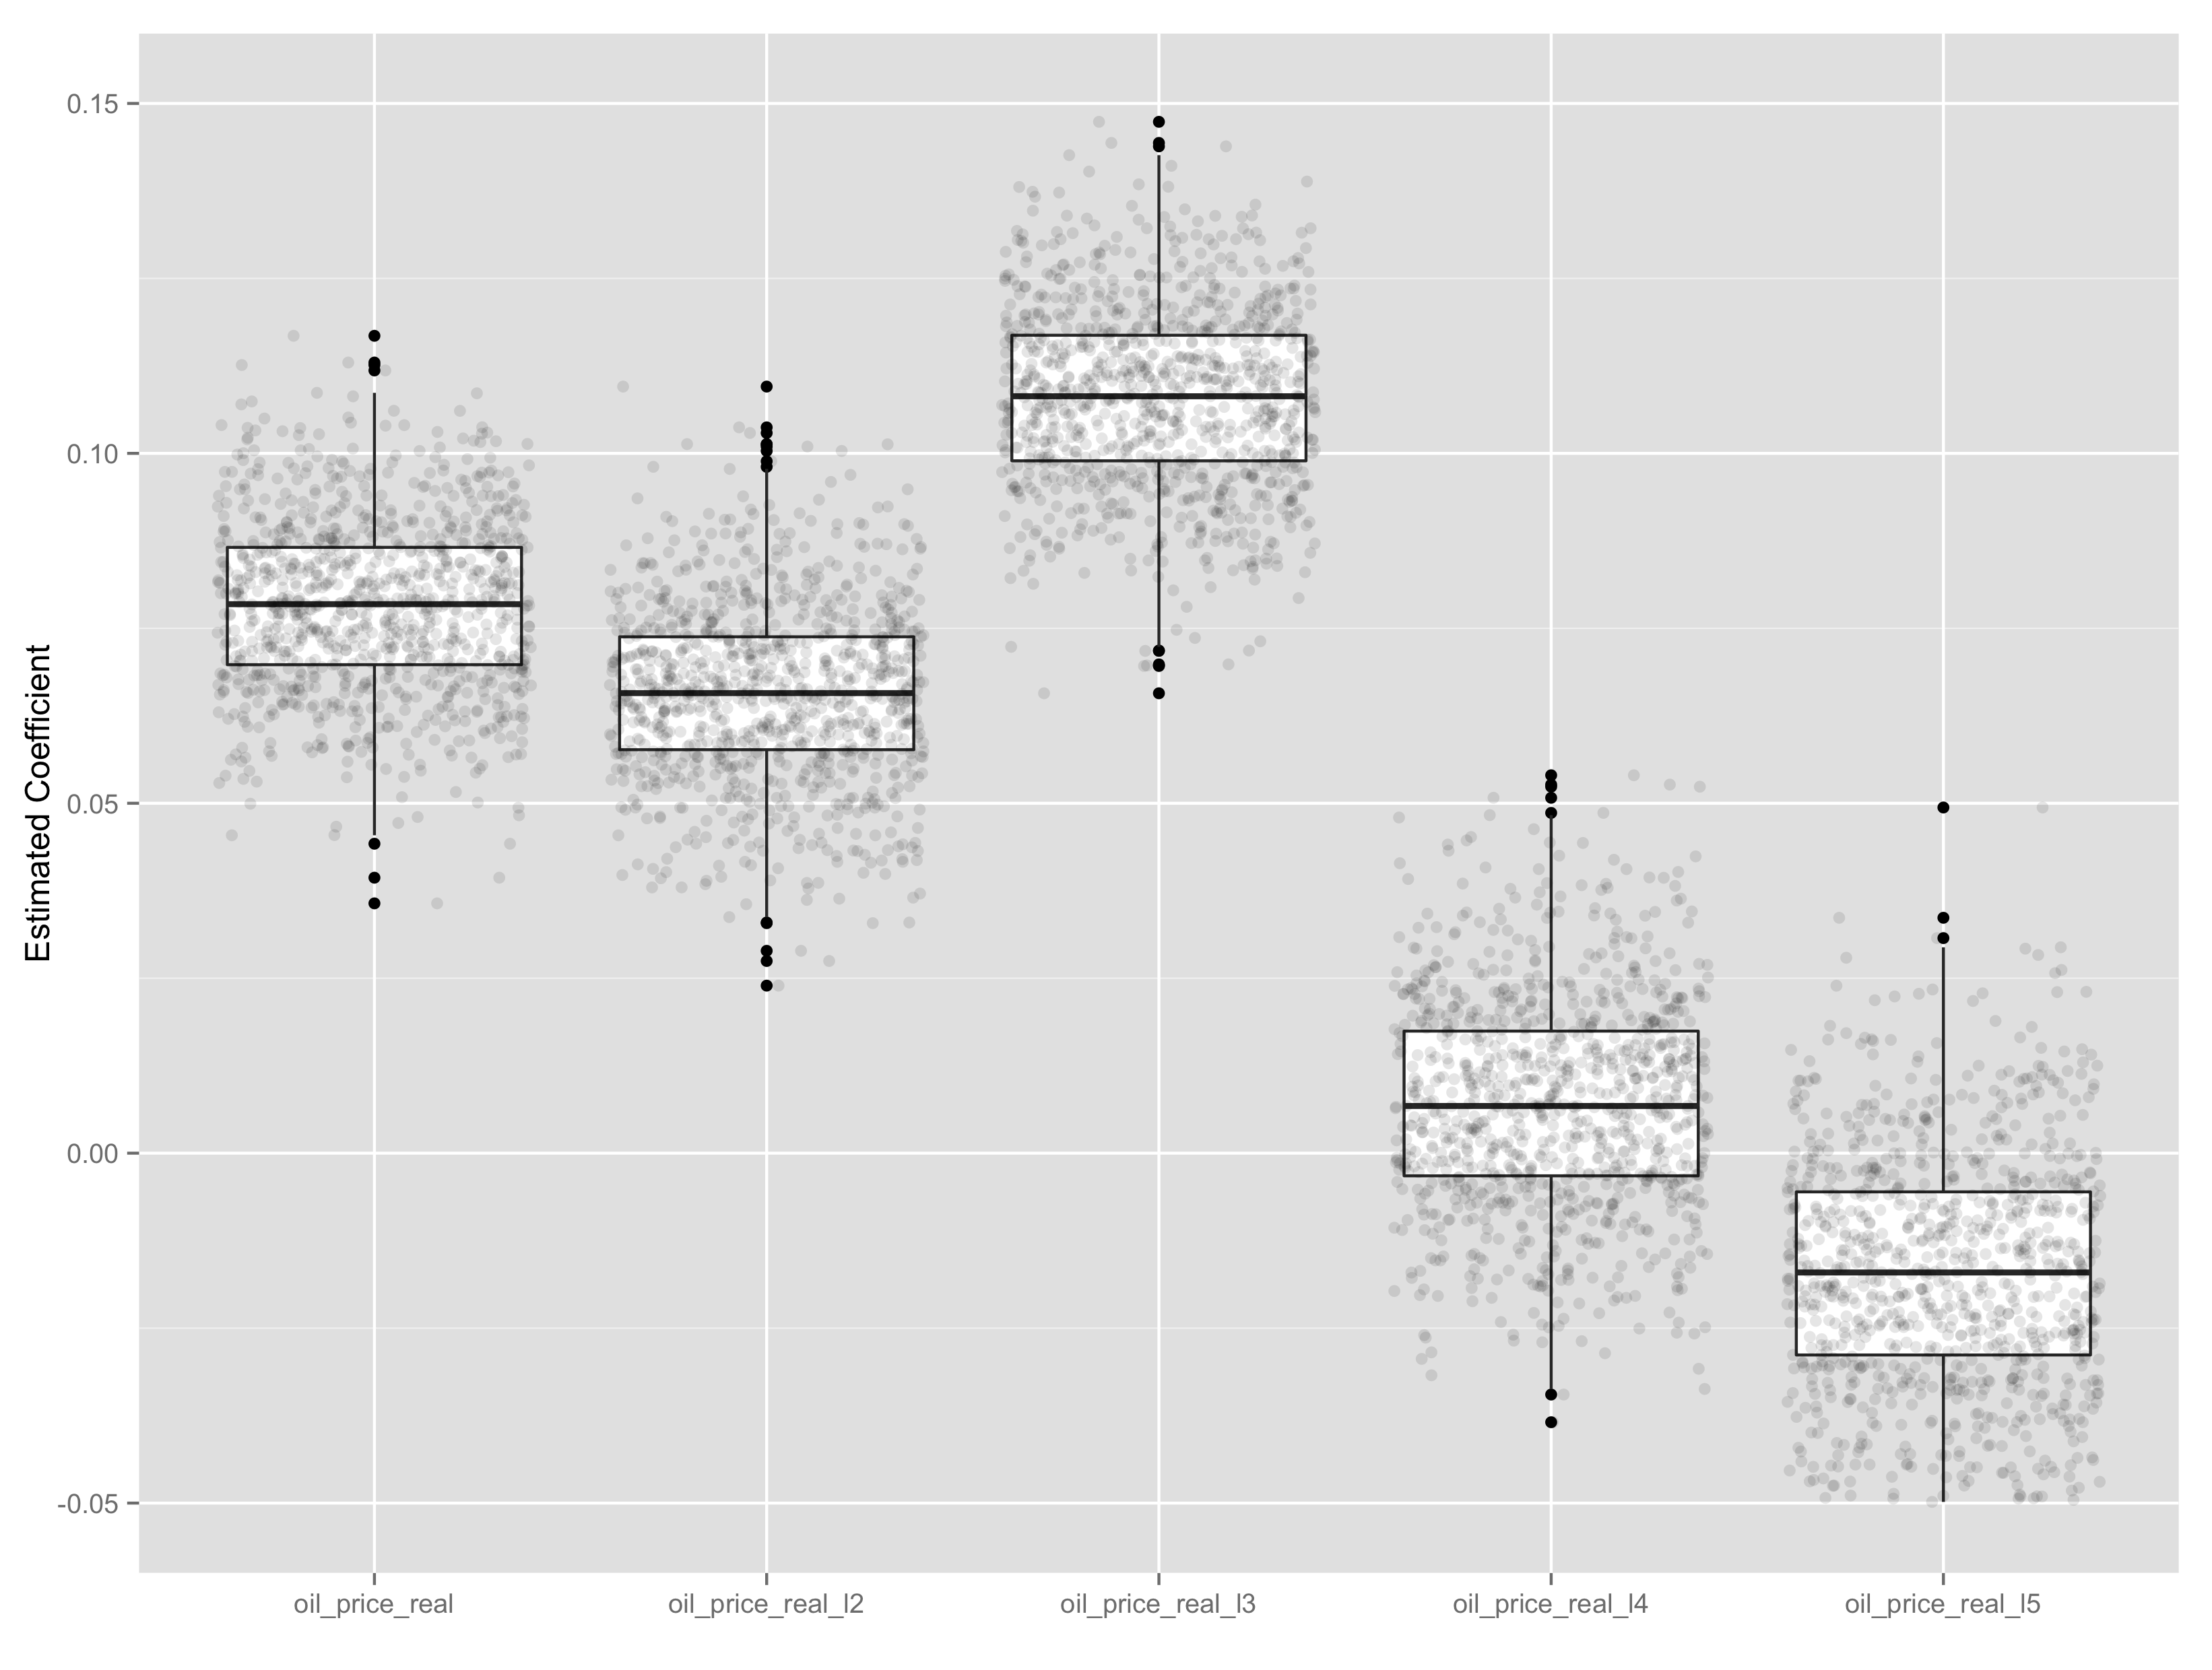
\includegraphics[width=.8\textwidth]{gam_price_invest_box.png}
	\caption{}
	\label{gam_price_invest_box}
\end{figure}

The results of the regression on investment fits nicely with the previous results on oil production which showed a significant effect in the 4th through 6th lags.  A story consistent with both results is that higher oil prices induce increased investment in production capacity, though it takes time to get the extra capacity in place and the effects on production to be felt.

\section{Conclusion}

\begin{figure}
	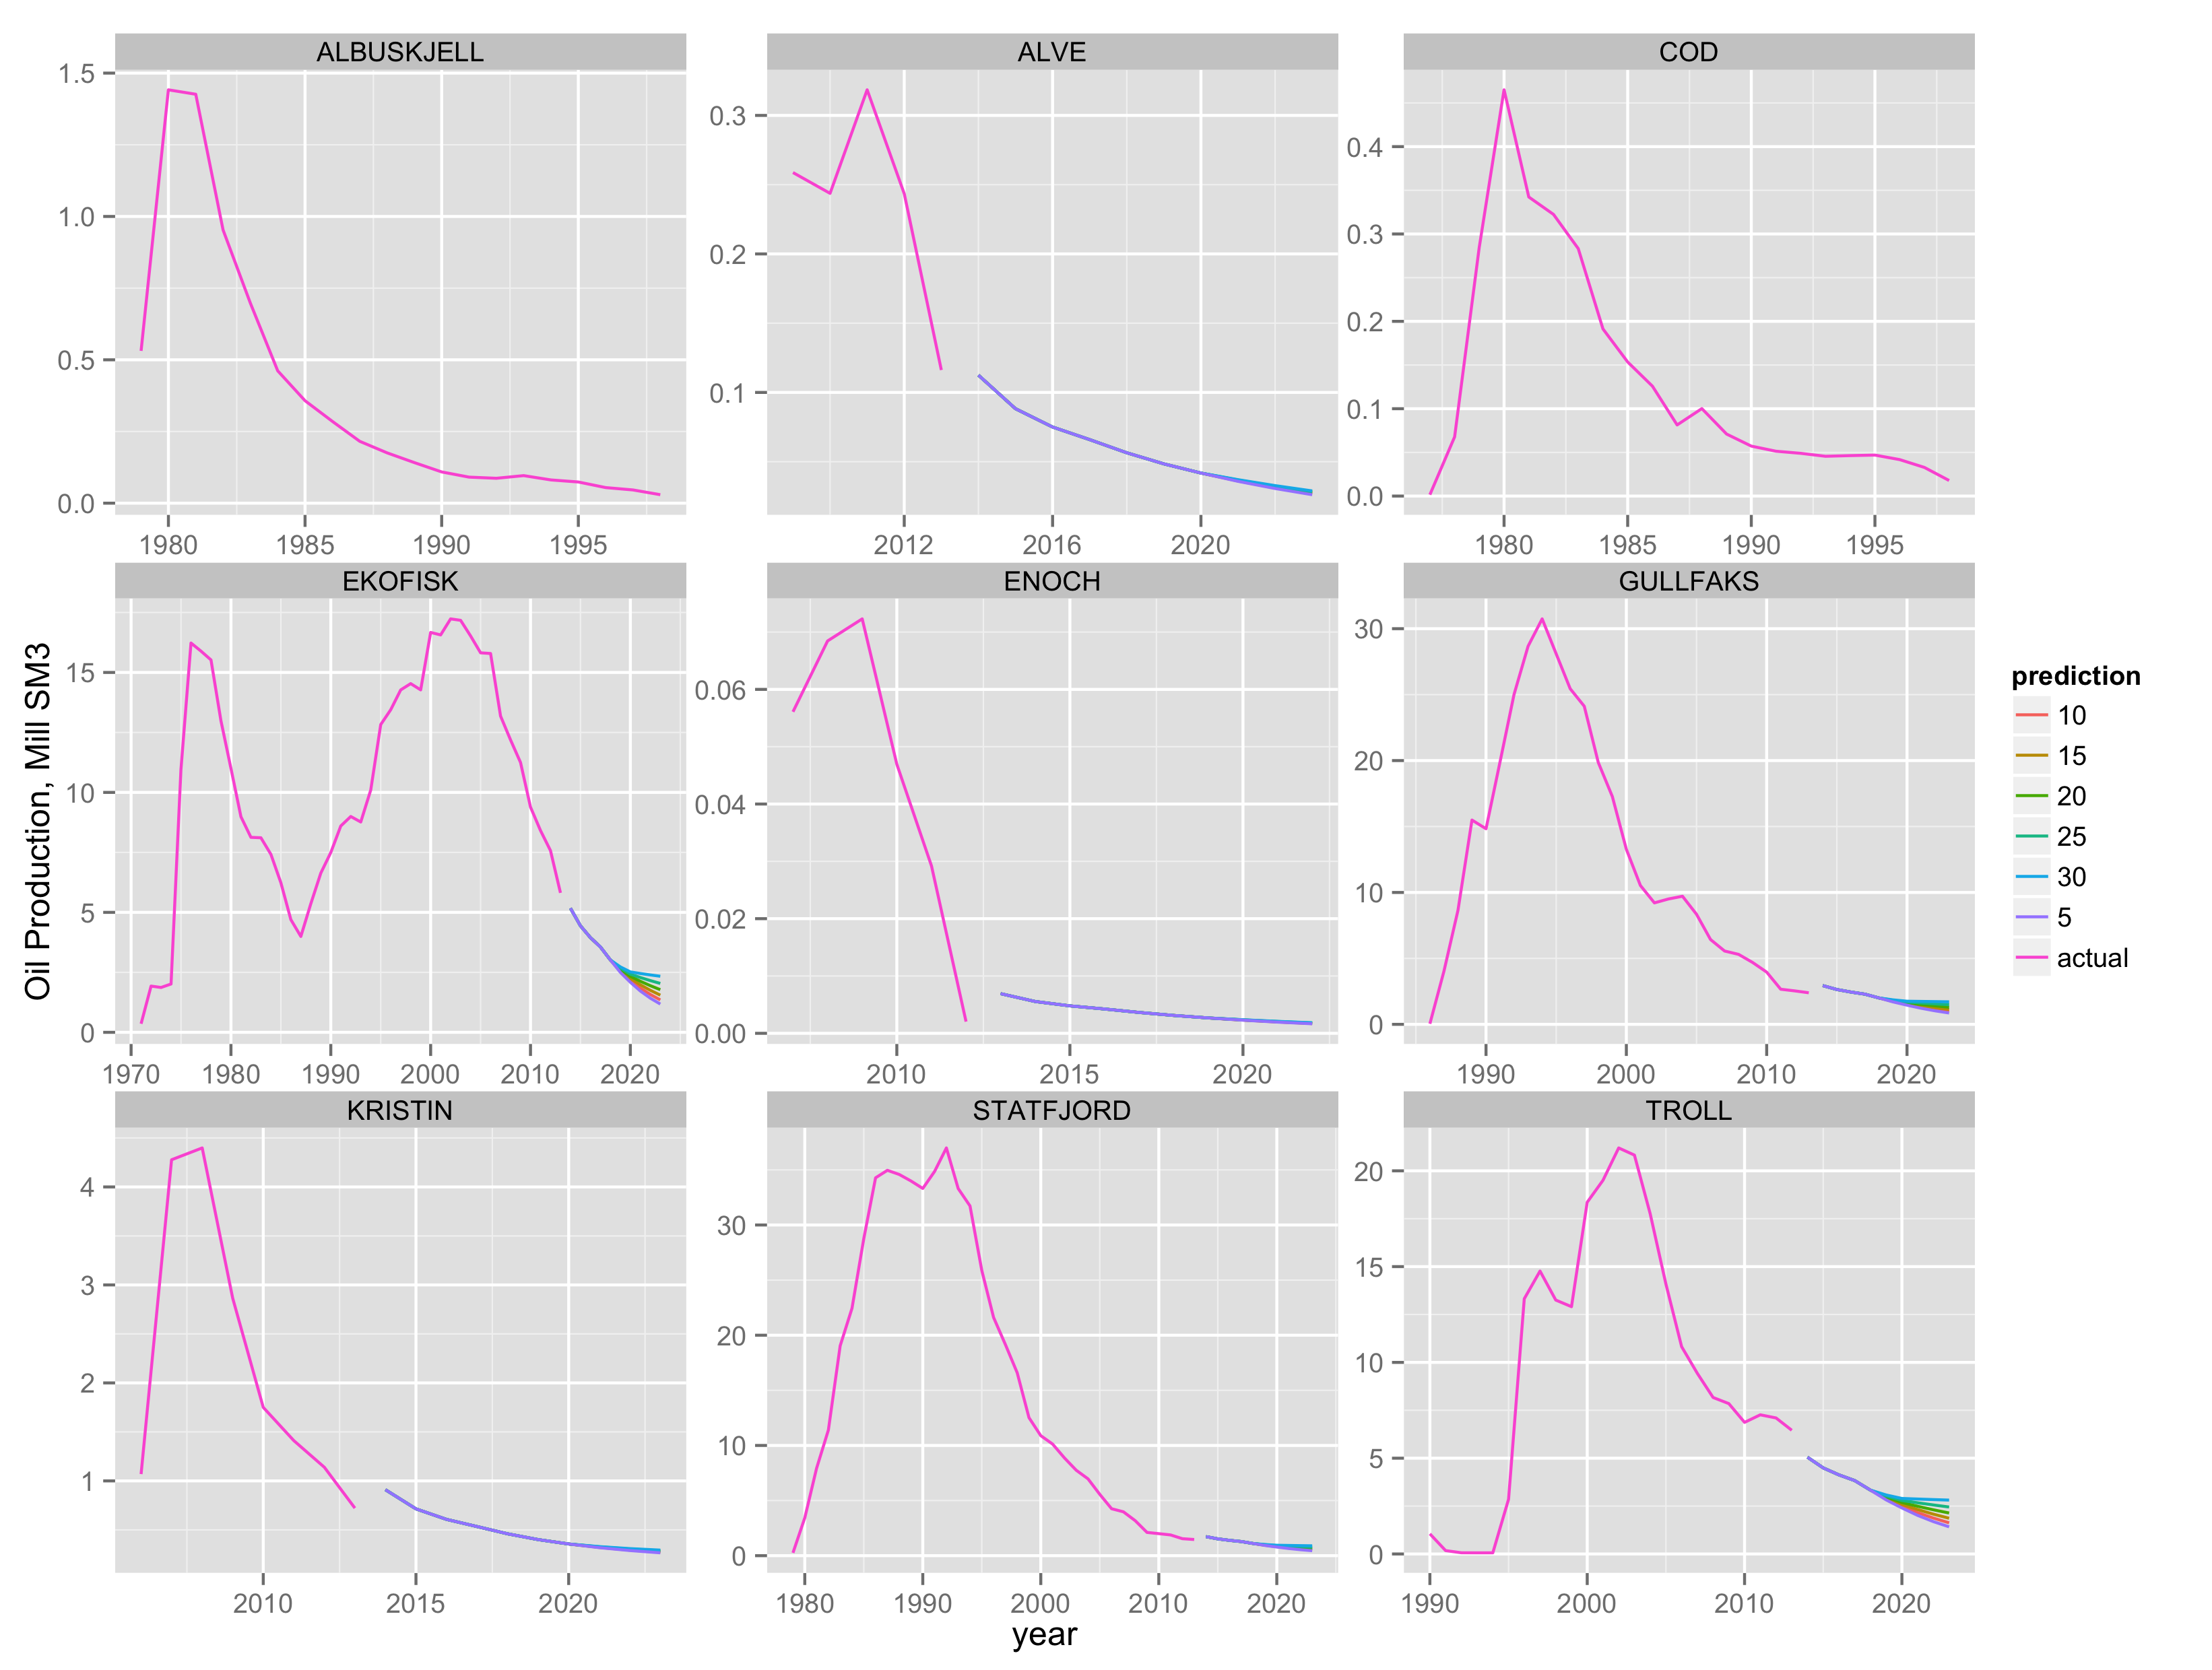
\includegraphics[width=.8\textwidth]{field_lev_forecast.png}
	\caption{}
	\label{field_lev_forecast}
\end{figure}

\begin{figure}
	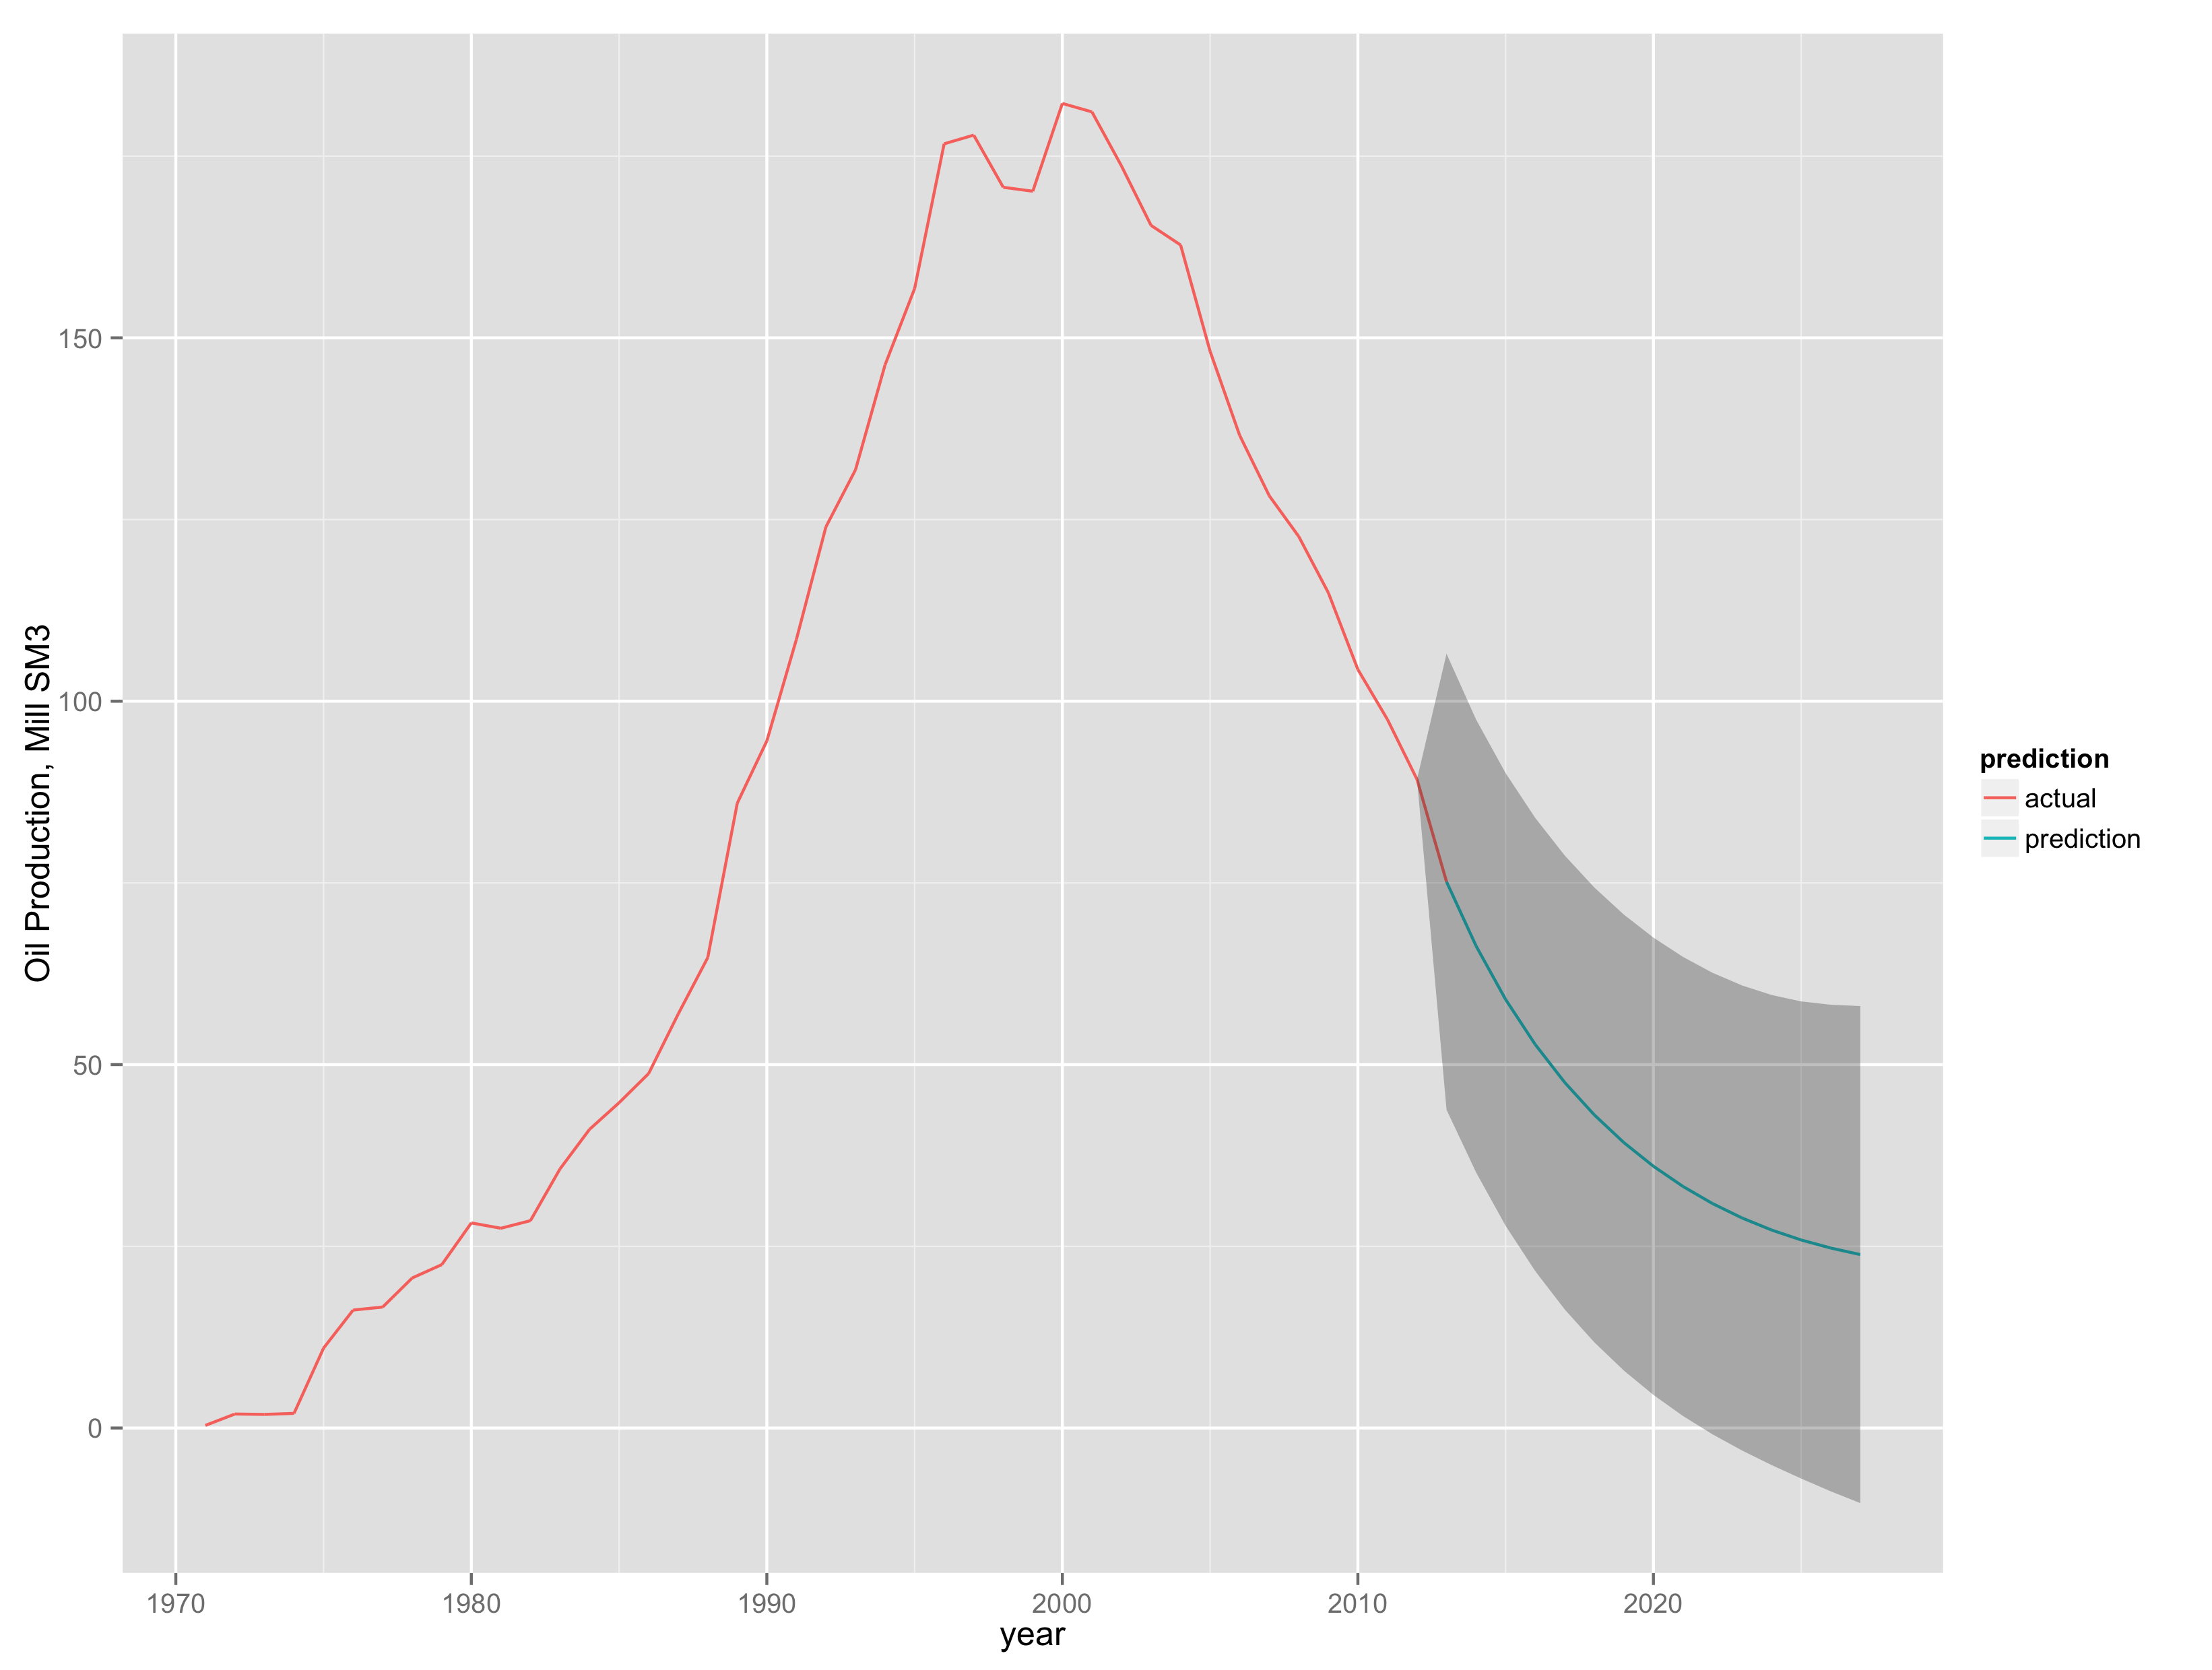
\includegraphics[width=.8\textwidth]{tot_forecast.png}
	\caption{}
	\label{tot_forecast}
\end{figure}

\begin{figure}
	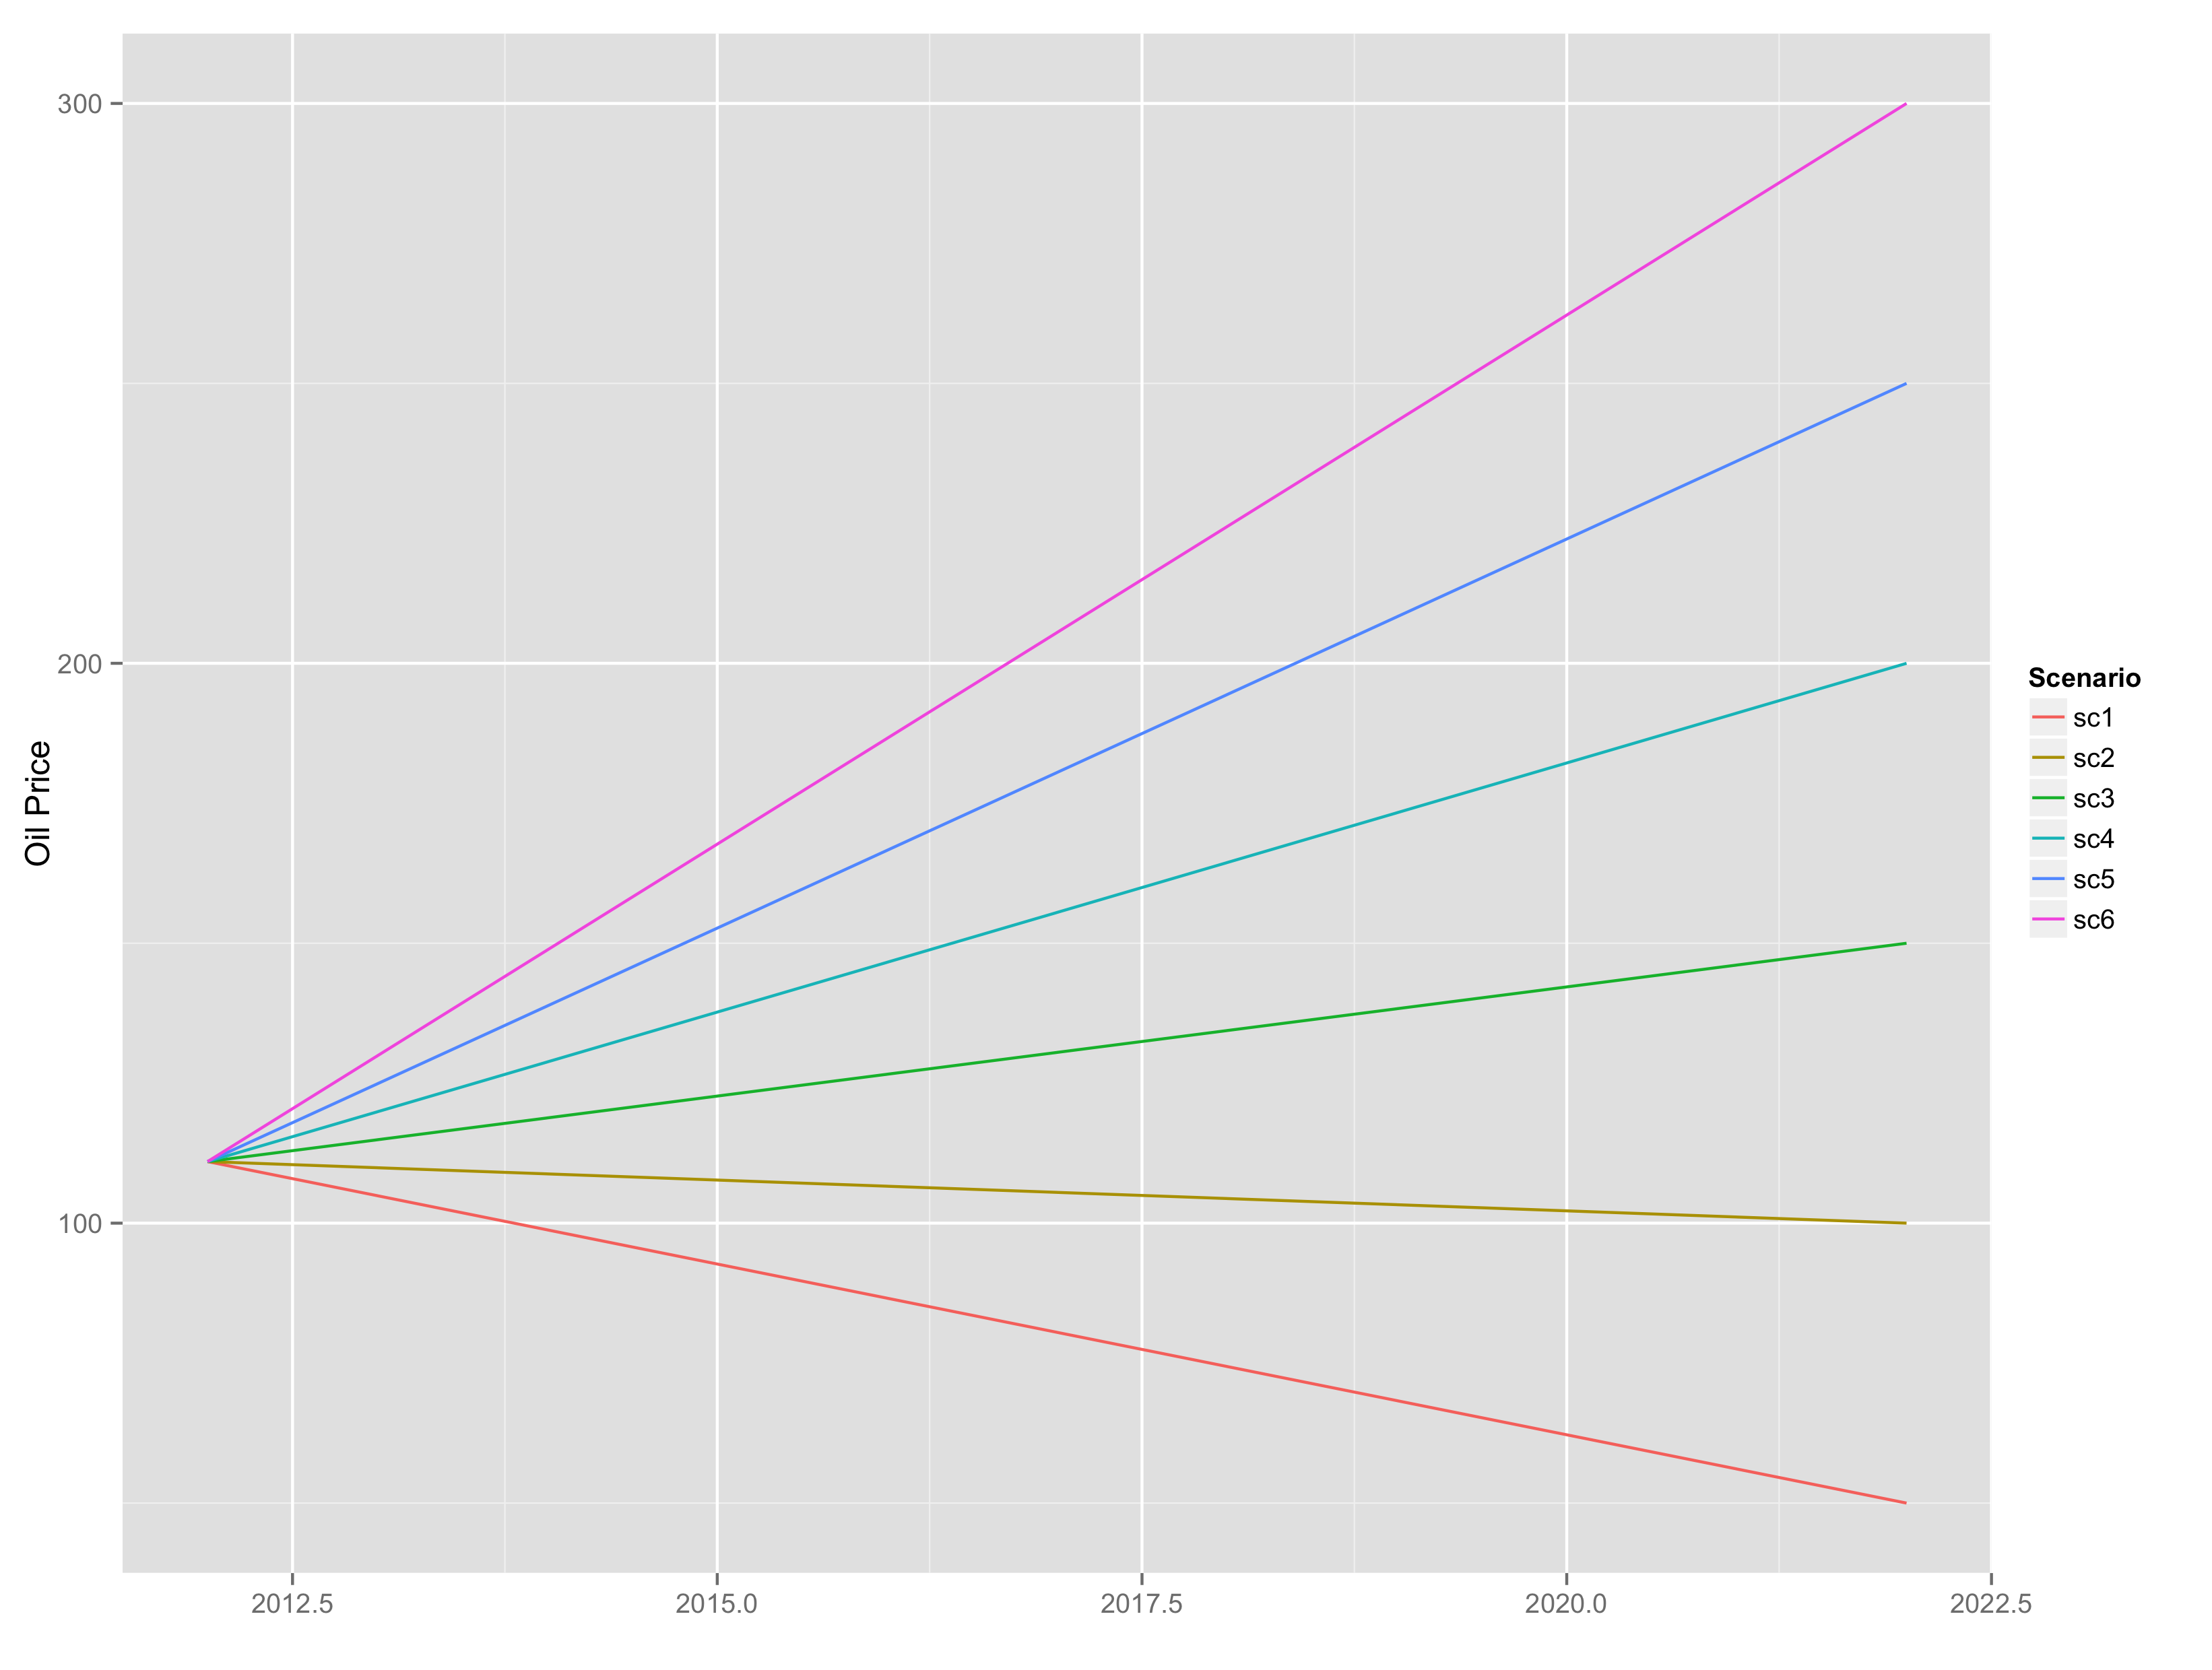
\includegraphics[width=.8\textwidth]{price_scenario.png}
	\caption{}
	\label{price_scenario}
\end{figure}

The results are important in themselves in helping explain and decompose the effect of price on oil production.  Production in existing fields has no significant concurrent reaction to higher oil prices while only slight lag of between 4 and 6 years is deducted.  Oil producers do not appear to be behaving strategically in relation to production - increasing or reducing production in response to changes in oil price.  Instead they are likely using storage or financial instruments to hedge price movements.  

Changes in oil prices can rather be seen as a relaxing of a production constraint, justifying increased investment that leads to either a higher total extraction rate or a intertemporal shifting of production.  

Beyond the explanatory importance of the papers results, the methodology - which to my knowledge have not been used in this field yet - can also serve a useful function in producing forecasts and scenarios.  The major advantage that the methodology has is that the estimates are based on field level approximations.  The empirical results from older fields are used to map forecasts of newer fields.  In this way, a forecast can be made that better fits the empirical shape of field-level production profiles.  

While a full forecasting model is outside the scope of this paper, I illustrate the potential with a simple forecast.  An important caveat here is that I am forecasting total oil production from existing fields.  Production from new fields are not estimated.  Figure \ref{field_lev_forecast} shows the forecast at the field level for several of the fields while figure \ref{tot_forecast} shows the aggregated forecast.  The different scenarios are for oil prices that increase or decrease by a fixed amount per year in order to read a certain oil price in the year 2022 as shown in figure \ref{price_scenario} .  

Visually, the forecasts appears sensible.  As would be expected from the results, the different oil price scenarios only lead to different outcomes after a several year delay.  An equally important point is how even a large difference in oil price leads to relatively minor change in expected production.   



\bibliographystyle{plainnat}
\bibliography{oil_prices}

\end{document}
This is never printed